\chapter{Selection and Categorisation}
\label{chap:selection_and_categorisation}

This thesis presents results of three different analyses used in the Higgs to two photon search at CMS. The nominal results and properties are obtained from the so-called \MFM analysis, which uses multivariate methods optimised specifically to search for a \SM Higgs boson to select and categorise events. This has a fully parametric definition of the diphoton invariant mass spectrum where the signal shape is derived from \MC simulation and the background shape from data. Events are selected by requiring that they pass a cut on the output of a \BDT trained to distinguish photons from jets (the \textit{photon ID BDT}) and furthmore that they pass a cut on an event level classifier (the \textit{diphoton BDT}) designed to collapse photon kinematics, mass resolution and photon quality into a single discriminating variable. Using the output of this event level classifier a number of analysis categories are defined to provide the optimal search sensitivty for a \SM Higgs boson. 

The second analysis is the \acf{SMVA} analysis which is a cut and count method and serves to cross check the background estimation in the \MFM analysis, the most significant unknown in a search like this, by extracting the background under the signal region from sidebands in the diphoton invariant mass spectrum. The \SMVA uses the same event selection as the \MFM although the categorisation is done differently. 

The third analysis is the \CiC analysis which is designed for simplicity and robustness as a cut based approach and, owing to its low level of model dependence, is used for statistical tests which attempt to ascertain the spin of the observed boson.

% ---- SECTION ----
\section{Event selection}
\label{sec:event_selection}

There are two complimentary event selections used in the three analyses. The \CiC analysis uses a cut-based photon selection whilst the \MFM and \SMVA analyses use a series of \BDTs to first select photons and then select events. The ultimate aim is a selection which accepts two prompt photons (i.e.\ does not contain any fakes) and exploits regions of phase space which have a narrow mass resolution and high signal to background ratio.

All events must contain at least two photons which pass $p_{T}^{\gamma_{1}}/m_{\gamma\gamma}>1/3$ (for the leading photon) and $p_{T}^{\gamma_{2}}/m_{\gamma\gamma}>1/4$ (for the subleading photon) and the invariant mass of the diphoton pair must be in the range $100<m_{\gamma\gamma}<180$~GeV. The reason for choosing \pT cuts which slide with \mgg is to avoid any Higgs mass, \mH, dependece in the selection. In the case where there are more than two photon candidates in an event, the two photons with the highest \pT are chosen. 

\subsection{Selection using cuts in categories}
\label{sec:cic}

The selection cuts are optimised for photons in four non-overlapping categories to take advantage of the different photon energy resolution between the barrel and the endcap and between converted and non-converted photons. The categories are defined as $|\eta|<1.444$ or $|\eta|>1.556$ (i.e.\ either barrel or endcap) and $R_{9}<0.94$ or $R_{9}\geq 0.94$ (i.e.\ either converted or non-converted) and the values for each of the cut variables (shown in Table~\ref{tab:cic_cuts}) are chosen by targeting a specific signal to background ratio ($S/B$). The procedure to define the cuts is as follows:

\begin{itemize}
  \item A set of loose cuts are defined as the starting values.
  \item The ``N-1" distribution of each cut variable is produced. This is the distribution of each variable after the cuts on all other variables have been applied.
  \item A smooth curve is fitted to the distribution of the $S/B$ ratio versus the cut variable.
  \item The cut value is chosen by evaluating the curve for the required value of $S/B$.
  \item Do the same for all the other variables.
\end{itemize}

Consequently a stable set of cut values is obtained by iterating this procedure a few times. Each cut will then select events with the same purity ($S/B$) and thus the efficiency for selected photons is maximised for the chosen purity level. As a result the cuts in the endcap are much tighter than in the barrel, similarly the cuts for low \rnine photons are much tighter than the cuts for high \rnine photons. The cut variables are described below and the cut values shown in Table~\ref{tab:cic_cuts}. The cut setting procedure is optimised on a signal sample of \Hgg \MC events (with \mH=120~\GeV) and a background sample of \gjet events. The photon efficiency of the cuts for the four different classes of photon is shown in Figure~\ref{fig:cic_efficiency} as a function of the supercluster position, \eta, and the photon \pT. The cut variables are:

\begin{itemize}
  \item PF isolation sum, chosen vertex - Sum of particle flow photon, charged and neutral hadron isolation sums defined in Sec.~\ref{sec:iso} where all \PF candidates originate from the primary vertex selected in Sec.~\ref{sec:vtx_reco}
  \item PF isolation sum, worst vertex - As above but where all \PF candidates originate instead from the vertex which gives the largest charged hadron PF isolation sum. This adds protection for cases when the primary vertex is incorrectly assigned.
  \item Charged PF isolation sum - Described above in Sec.~\ref{sec:iso}.
  \item $\sigma_{i\eta i\eta}$ - Described above in Sec.~\ref{sec:photon_presel}.
  \item $H/E$ - Described above in Sec.~\ref{sec:photon_presel}.
  \item $R_{9}$ - Described above in Sec.~\ref{sec:ecal}.
\end{itemize}

\begin{table}
  \begin{center}
    \begin{tabular}{l l l l l}
      & \multicolumn{2}{c}{Barrel} & \multicolumn{2}{c}{Endcap} \\ 
      & \multicolumn{1}{l}{\rnine $\geq$ 0.94} & \multicolumn{1}{l}{\rnine $<$ 0.94 } & \multicolumn{1}{l}{\rnine $\geq$ 0.94 } & \multicolumn{1}{l}{\rnine $<$ 0.94 } \\ 
      \hline
      PF isolation sum, chosen vertex (GeV) & $<$6 & $<$4.7 & $<$5.6 & $<$3.6 \\ 
      PF isolation sum, worst vertex (GeV) & $<$10 & $<$6.5 & $<$5.6 & $<$4.4 \\ 
      Charged PF isolation sum (GeV) & $<$3.8 & $<$2.5 & $<$3.1 & $<$2.2 \\ 
      $\sigma_{i\eta i\eta}$ & $<$0.0108 & $<$0.0102 & $<$0.028 & $<$0.028 \\ 
      H/E & $<$0.124 & $<$0.092 & $<$0.142 & $<$0.063 \\ 
      \rnine & $>$0.94 & $>$0.298 & $>$0.94 & $>$0.24 \\ 
    \end{tabular}
  \end{center}
  \caption{Photon ID selection cut values. The cuts are applied to both the leading and subleading photons.}
  \label{tab:cic_cuts}
\end{table}

\begin{figure}
  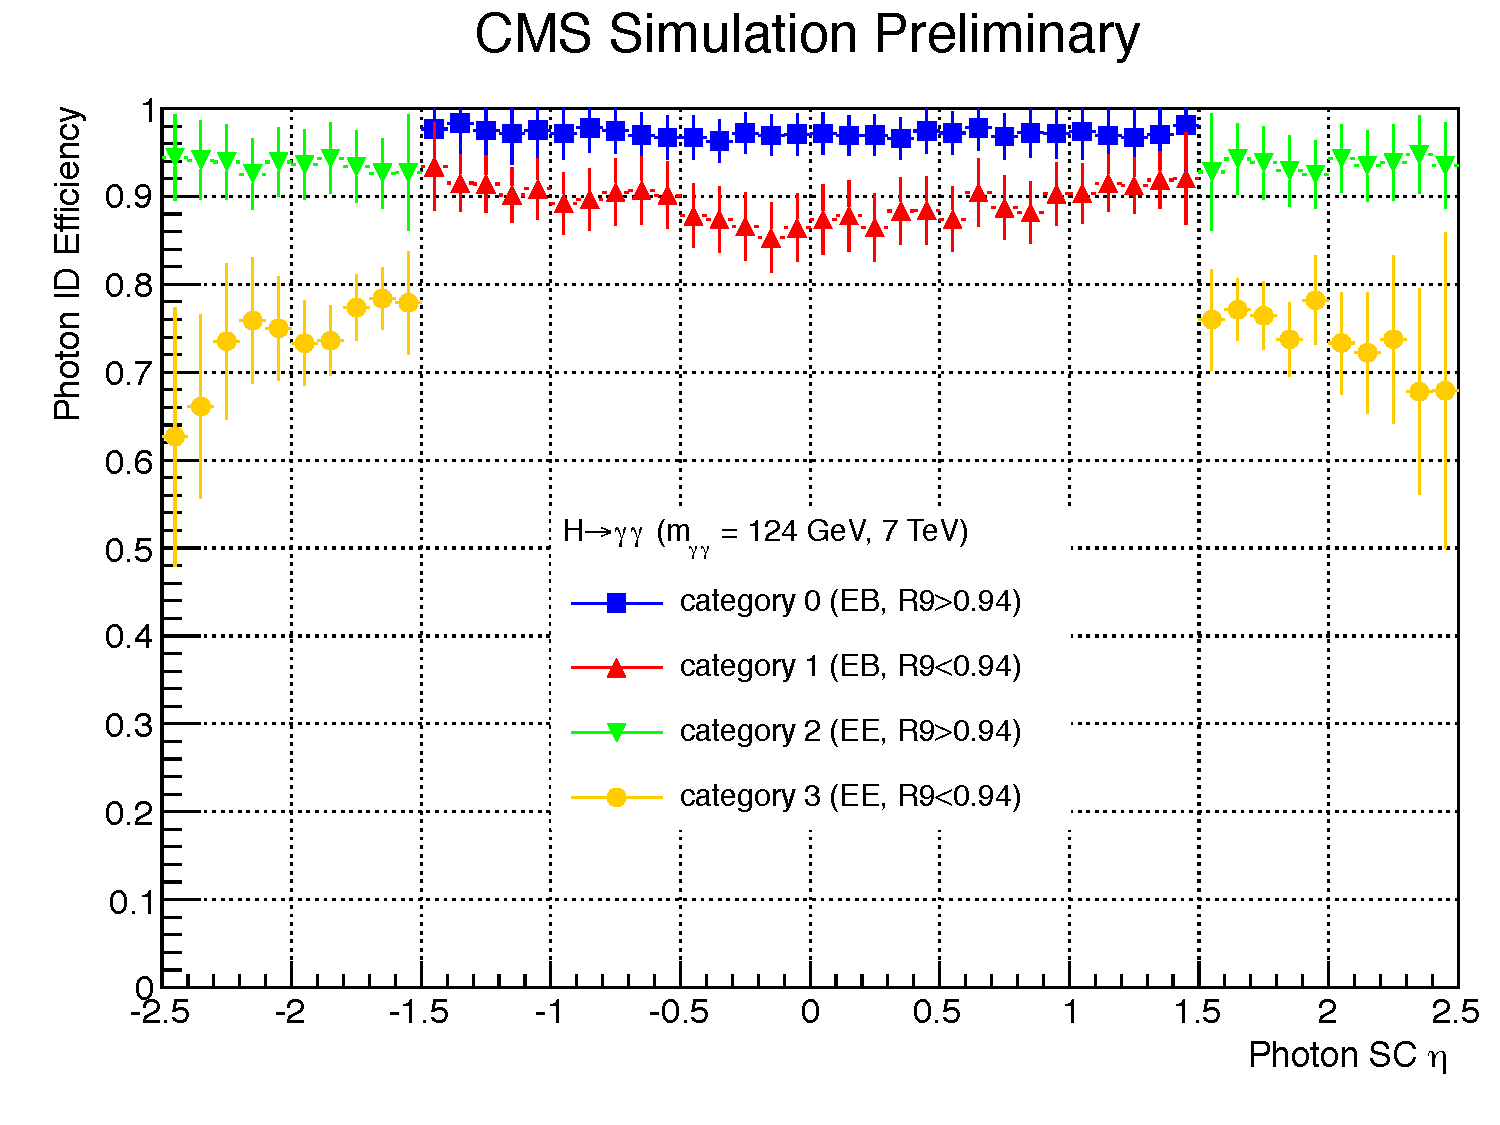
\includegraphics[width=0.49\textwidth]{selec_and_cats/plots/eff_7TeV_eta_fix.pdf}
  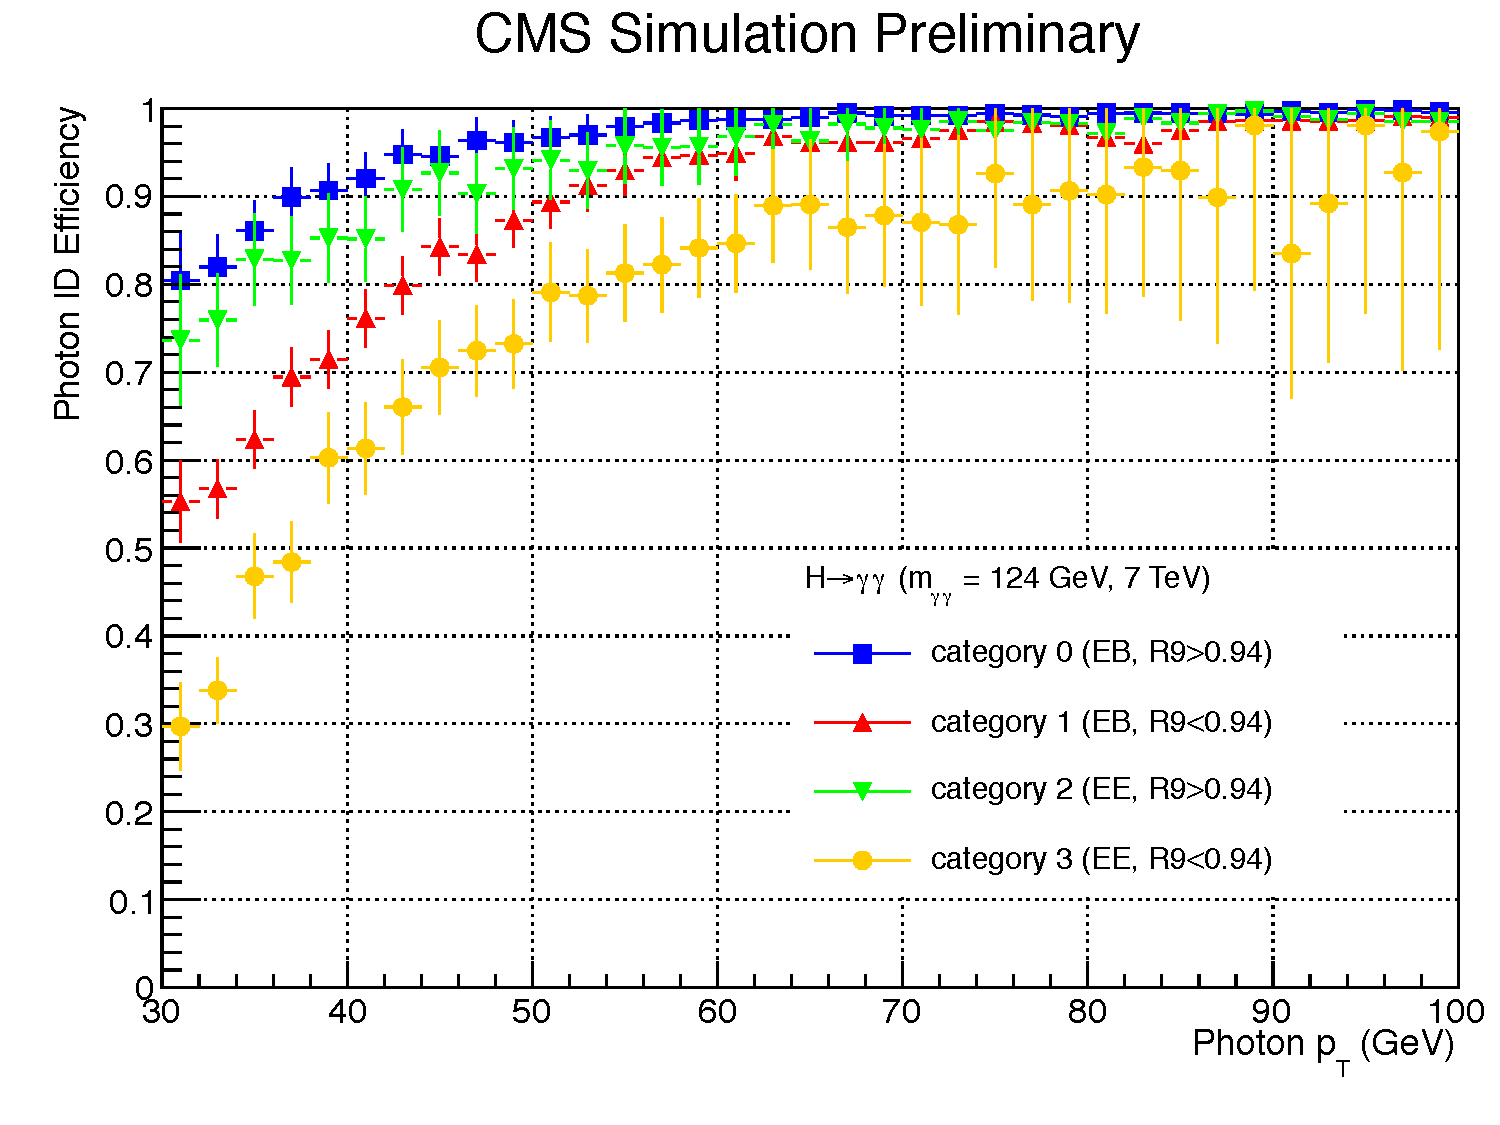
\includegraphics[width=0.49\textwidth]{selec_and_cats/plots/eff_7TeV_pt_fix.pdf}
  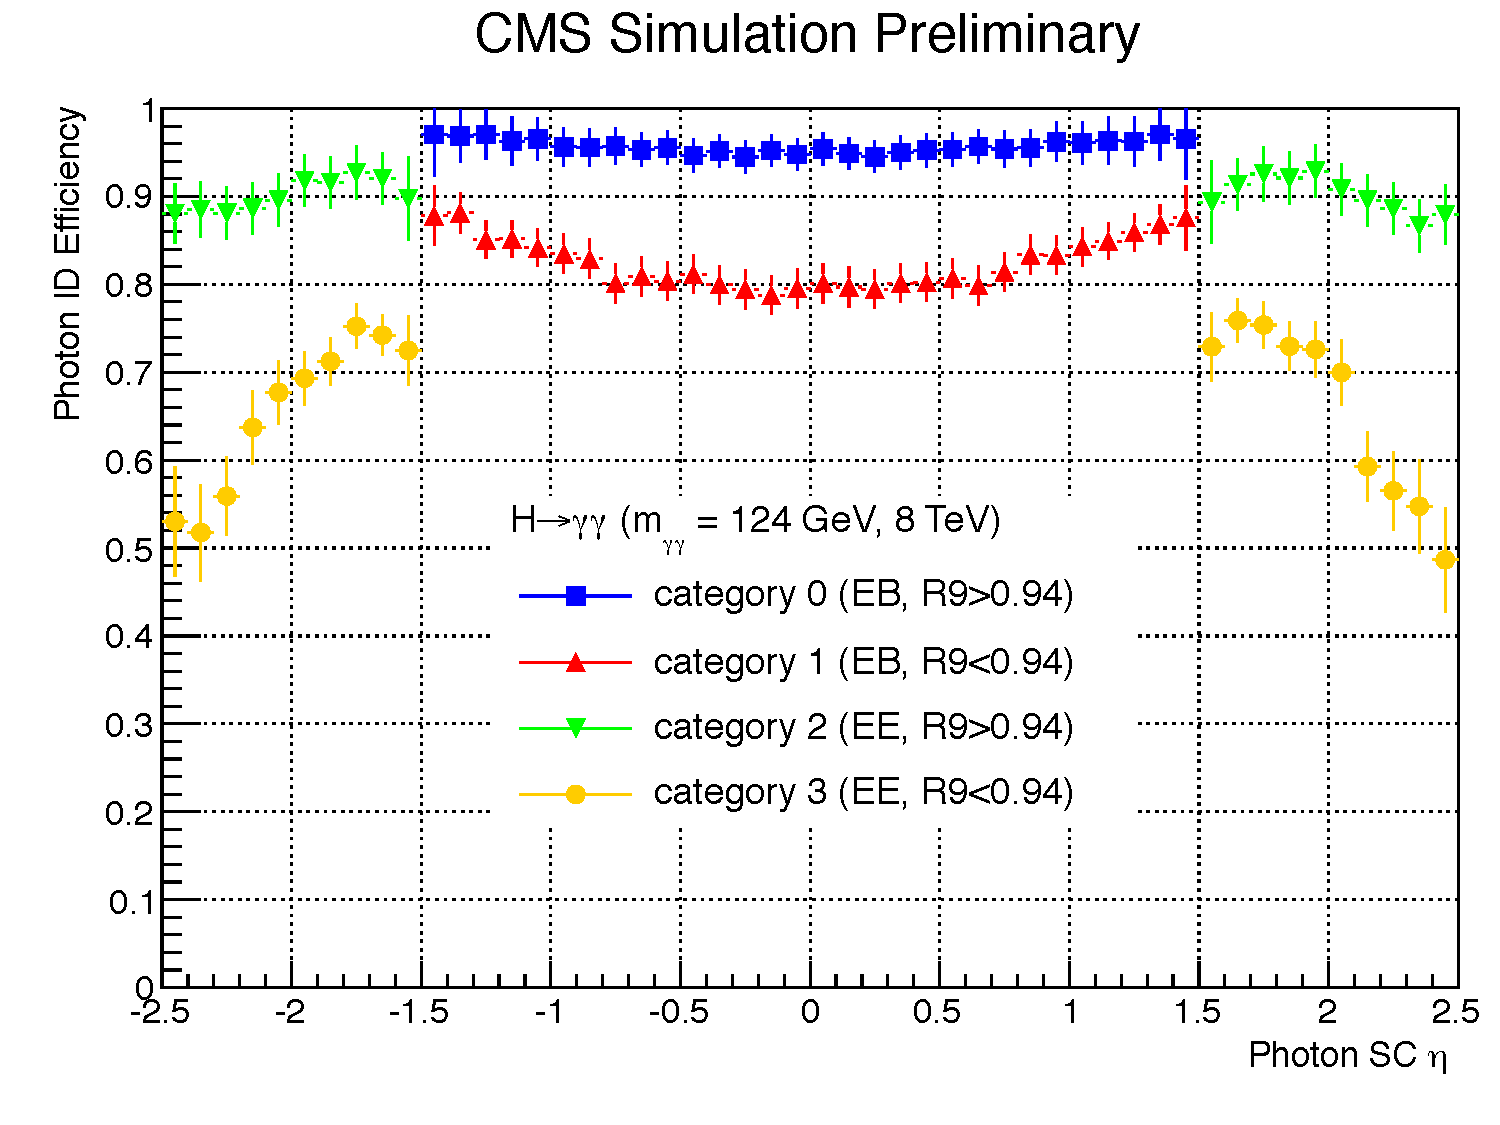
\includegraphics[width=0.49\textwidth]{selec_and_cats/plots/eff_8TeV_eta_fix.pdf}
  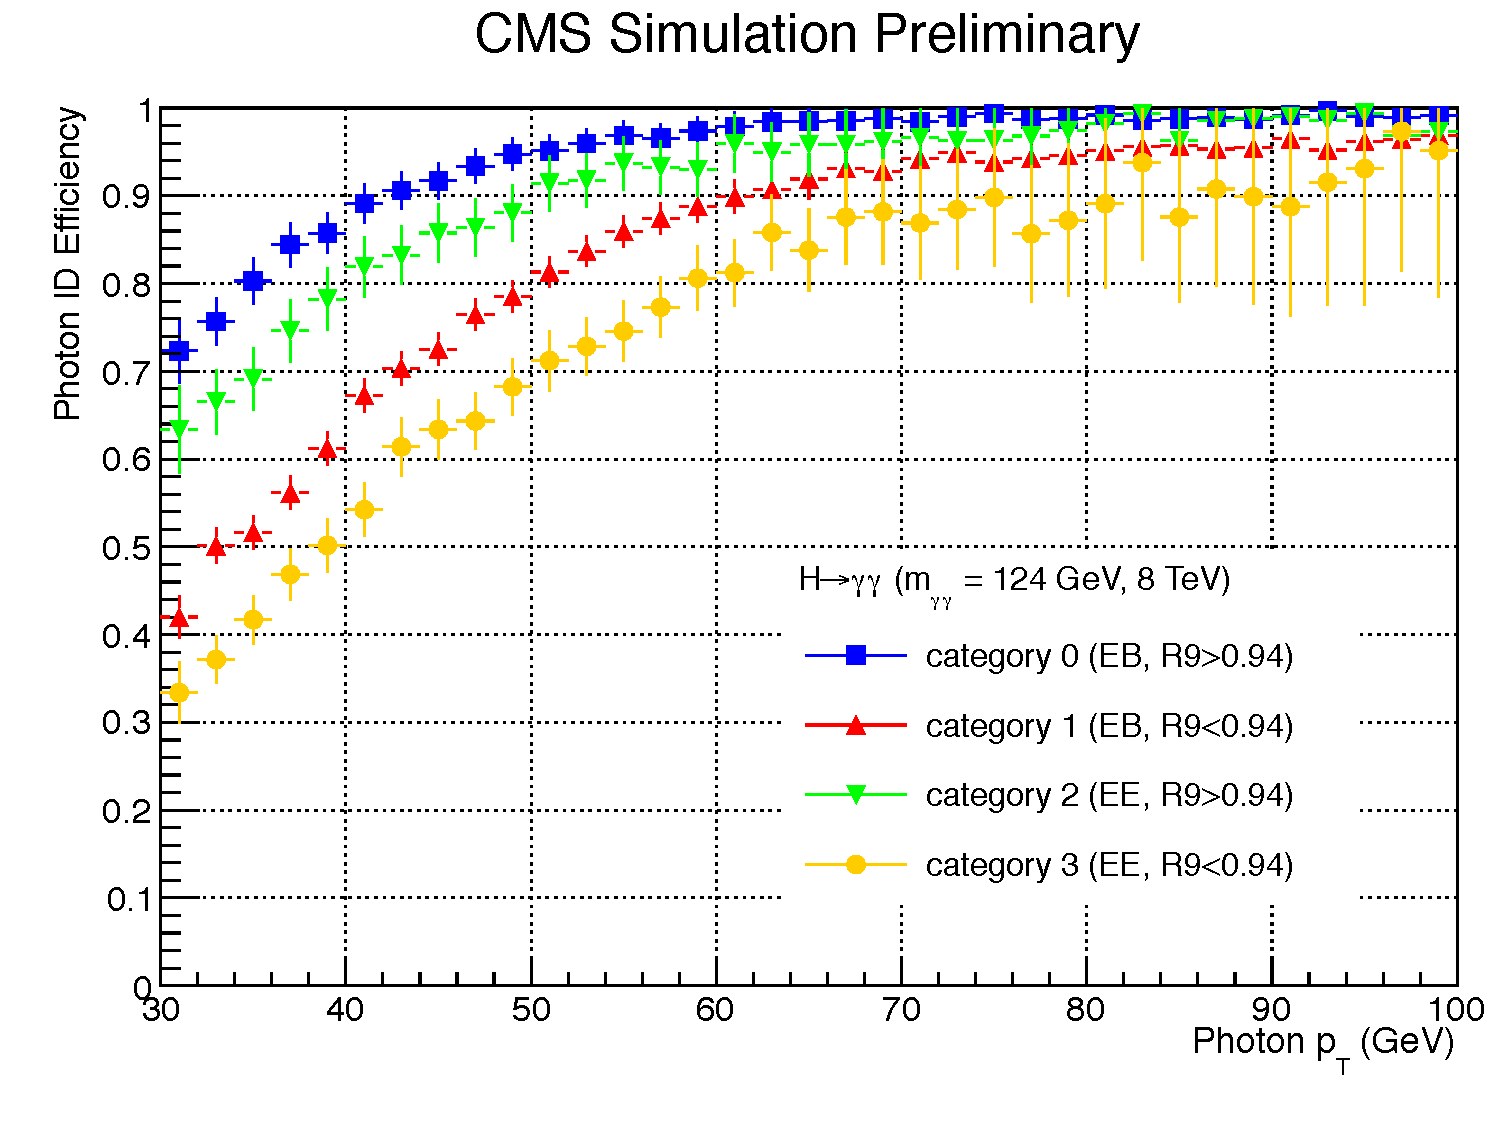
\includegraphics[width=0.49\textwidth]{selec_and_cats/plots/eff_8TeV_pt_fix.pdf}
  \caption[Cut based photon ID efficiency as measured in \Zee \acs{MC} simulation]{Cut based photon ID efficiency as measured in \Zee \MC simulation using the tag and probe method~\cite{tag_and_probe}. Shown for the 7~TeV dataset (top row) and 8~TeV dataset (bottom row) as a function of the photon supercluster position in \eta (left) and as a function of the photon \pT (right). Photons in the barrel which are unconverted (converted) are plotted as the blue (red) points and photons in the endcap which are unconverted (converted) are plotted as the green (yellow) points.}
  \label{fig:cic_efficiency}
\end{figure}

\subsection{Photon ID MVA}
\label{sec:pho_id_mva}

For the \MFM and \SMVA analyses a \BDT is trained to discriminate between prompt photons and jets. The desire is to factorise the photon selection, which is required to distinguish prompt photons from neutral mesons faking photons, and the event selection, which is required to consider kinematics, resolution, etc.~to distinguish \Hgg from the $pp\rightarrow\gamma\gamma$, \gjet, $\mathrm{jet}+\mathrm{jet}$ background. The input variables used are designed specifically to distinguish between photons and fakes. They should not have any properties which make the identification Higgs specific. Consequently, the training samples used are \gjet samples where the identification \BDT signal is the prompt $\gamma$ and the background is the fake jet. The \pT and supercluster \eta distributions are reweighted such that they match between signal and background. This negates the \BDT exploiting any photon kinematics which could correlate to the Higgs mass. The photon ID \BDT is trained separately for the barrel and endcap as these regions of phase space are so different. Seperate \BDTs were also trained for 7 and 8~TeV. The result is four separate trainings in total.

The input variables aim to exploit differences in the shower shape and isolation between prompt and non-prompt photons and the correlation between these variables and the supercluster position and energy. They are:

\noindent\textbf{Shower shape variables}
\begin{itemize}
  \item $\sigma_{i\eta i\eta}$ - Explained above in Sec.~\ref{sec:photon_presel}.
  \item $\sigma_{i\eta i\phi}$ - The equivalent diagonal spread (in \eta,\phi), representing the ($\eta$,$\phi$) correlation of the shower.
  \item $E_{2\times2}/E_{5\times5}$ - Ratio of the energy in the most energetic 2$\times$2 cluster which contains the seed to the energy in the 5$\times$5 cluster.
  \item $R_{9}$ - Explained above in Sec.~\ref{sec:ecal}.
  \item $\sigma_{\eta}$ - The energy weighted standard deviation of single crystal \eta within the supercluster.
  \item $\sigma_{\phi}$ - The energy weighted standard deviation of single crystal \phi within the supercluster.
  \item $\sigma_{xy}$ (for endcap only) - The standard deviation of the shower spread in the $x$, $y$ planes of the preshower, representing the $x$-$y$ correlation of the shower.
\end{itemize}

\noindent\textbf{Isolation variables}
\begin{itemize}
  \item PF Photon ISO - Particle flow photon isolation sum.
  \item PF Charged Hadron ISO (selected vertex) - Particle flow charged hadron isolation sum for candidates originating from selected vertex.
  \item PF Charged Hadron ISO (worst vertex) - Particle flow charged hadron isolation sum for candidates originating from the vertex with the largest isolation sum.
\end{itemize}

\noindent\textbf{Correlation variables}
\begin{itemize}
  \item $\rho$ - The median energy density in the event.
  \item $\eta$ - The \eta position of the photon supercluster.
  \item $E_{raw}$ - The raw energy of the photon supercluster.
\end{itemize}

The testing sample used to verify the output of the photon identification \BDT is a \MC \Hgg sample (\mH=124~\GeV). The photon identification \BDT output provides a measure of an individual photon's ``quality" and is used as an input to the event level \BDT (described in the next section). Even so, a considerable amount of background is cut out by defining a loose cut (the \BDT output must be $>-0.2$) on the photon ID \BDT output value which is more than 99\% signal efficient. This is demonstrated in Fig.~\ref{fig:photon_id_bdt} which shows the photon ID \BDT output for a \Hgg signal \MC sample and for all the data events which pass the preselection defined in Sec.~\ref{sec:photon_presel}. It is clear that placing a cut at $>-0.2$ removes a considerable amount of the background whilst maintaining very high signal efficiency. 

The photon ID \BDT response for each photon is used as a direct input to the event level \MVA. Given that imperfect modeling of the detector response can result in a small change in the photon ID response which has a direct impact on the event level \MVA response, which is used to classify events, a systematic error on the photon quality is applied and propagated through to the event level \MVA. Validation of the photon ID \BDT response in the \Zee decay is shown in Fig.~\ref{fig:photon_id_zee} with the size of the systematic error applied to account for any data/\MC discrepancies. The uniform response of the identification as a function of the number of primary vertices is demonstrated by the similarity of the two plots in this figure (Fig.~\ref{fig:photon_id_zee}) which are for events in which the number of primary vertices is $\leq 15$ (on the left) and for those in which the number of primary vertices is $>15$ (right).

\begin{figure}
  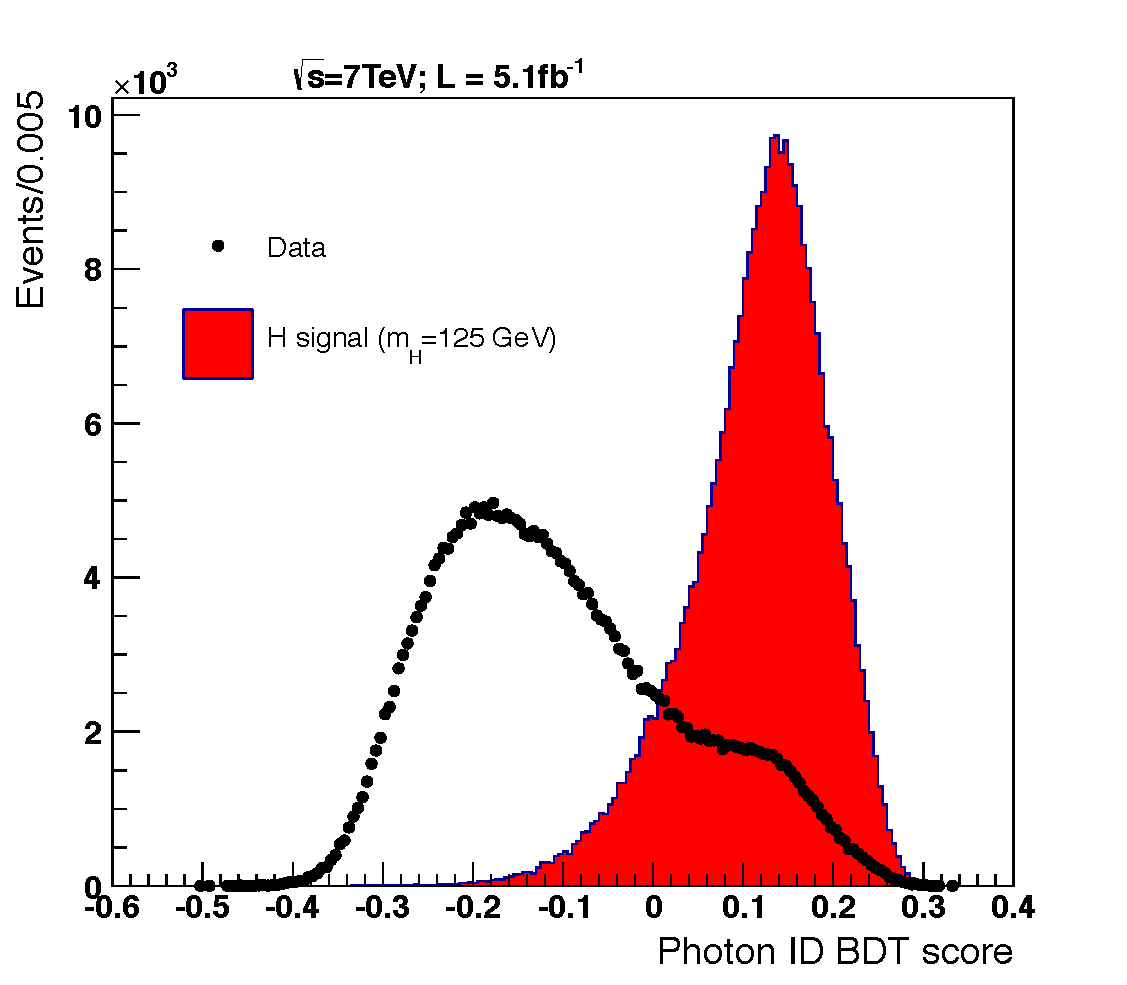
\includegraphics[width=0.48\textwidth]{selec_and_cats/plots/lowScoreID_7TeV_fix.pdf}
  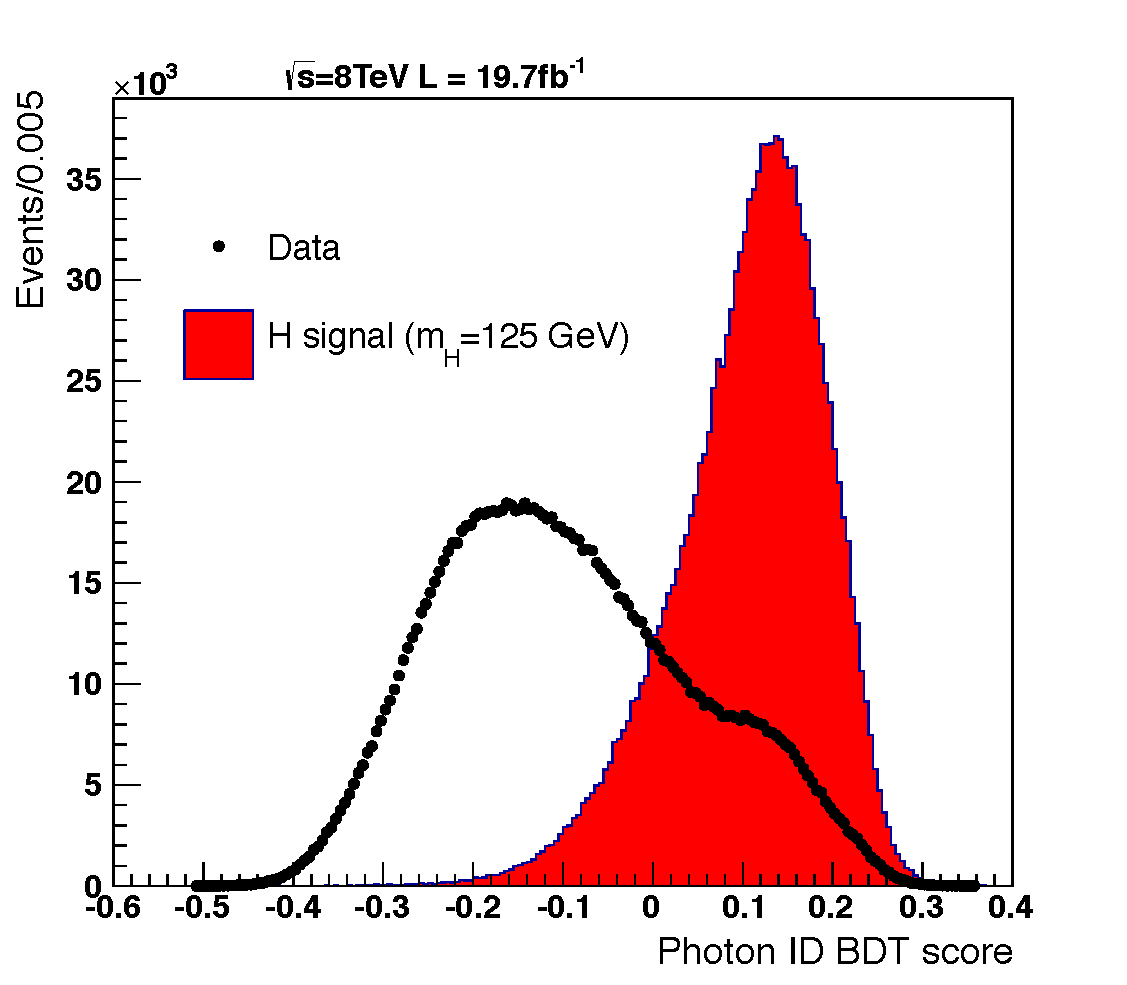
\includegraphics[width=0.48\textwidth]{selec_and_cats/plots/lowScoreID_8TeV_fix.pdf}
  \caption[The output distribution of the photon identification \acs{BDT}]{The output distribution of the photon identification \BDT for 7~\TeV (left) and 8~\TeV (right) datasets. The black points show the output for data events which pass the preselection and the red histogram shows the output for a simulated \MC sample of \Hgg decays. A cut of $>-0.2$ is made on all photons.}
  \label{fig:photon_id_bdt}
\end{figure}

\begin{figure}
  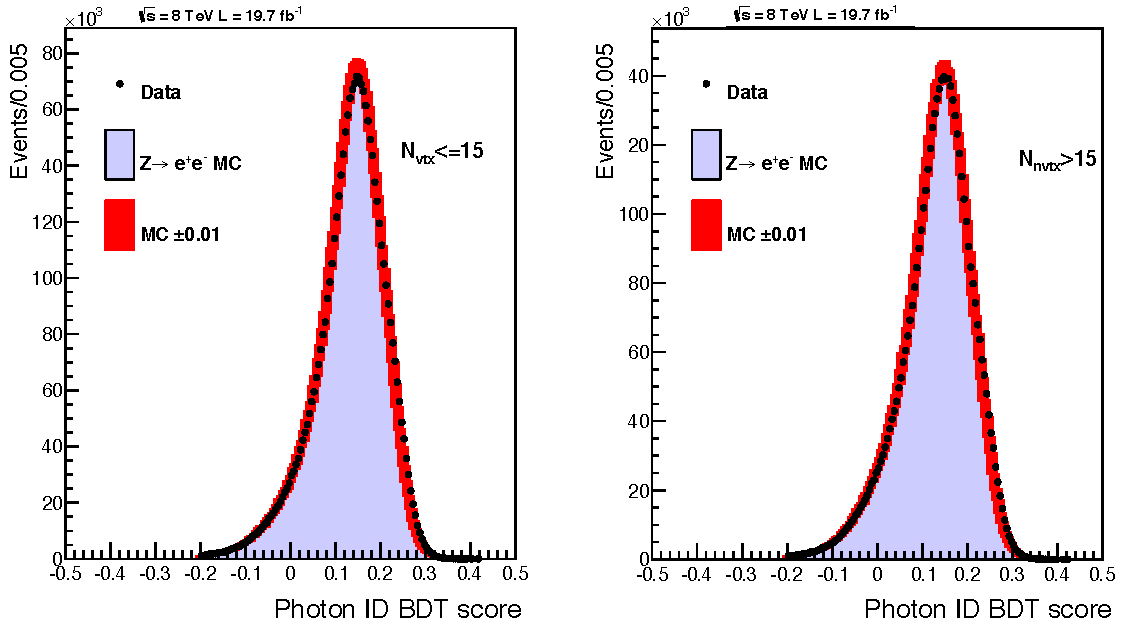
\includegraphics[width=0.98\textwidth]{selec_and_cats/plots/idmva_nvtx_fix.pdf}
  \caption[The output distribution of the photon identification \acs{BDT} in \Zee decays]{The output distribution of the photon identification \BDT for the 8~\TeV training as validated by the \Zee decay for events which have $\leq15$ reconstructed primary vertices (left) and those which have $>15$ primary vertices (right). The data is shown as the black points with the \MC simulation as the blue histogram. The systematic uncertainty on the output as applied to the \MC sample is shown as the red band.}
  \label{fig:photon_id_zee}
\end{figure}

\subsection{Diphoton event level MVA}
\label{sec:diphoton_bdt}

Whilst the CiC analysis selects events based on photon identification, the \MVA analysis approach is to first select photons using the photon identification \BDT described in the section above and then pass all the relevant event information through an event level \BDT. The event level classifier, referred to as the diphoton \BDT, is constructed to give a high score to events which fulfill the following criteria:

\begin{enumerate}
  \item The event kinematics should be compatible with a Higgs decay.
  \item The event has good mass resolution.
  \item The event contains two ``high quality" photons (i.e.~they have a high score from the photon ID \BDT).
\end{enumerate}

It is highly important that the \BDT is completely independent of Higgs mass and consequently that the input variables have no, or at the least very little, dependence on the Higgs mass. This is essential to have a fair training. If the \BDT included the Higgs mass, or a variable highly correlated with it, it would preferentially select events with this mass therefore biasing the selection towards events which have a mass near the mass of the signal used to train with. The input variables used are:

\noindent\textbf{Event kinematics}
\begin{itemize}
  \item $p_{T}^{1(2)}/m_{\gamma\gamma}$ - The mass relative transverse momenta of each photon.
  \item $\eta^{1(2)}$ - The pseudorapidity of each photon.
  \item $\cos(\phi_{1}-\phi_{2})$ - The cosine of the angle between the two photons in the transverse plane. This variable reflects the \pT of the diphoton system (in other words the reconstructed Higgs candidate) without introducing a mass dependence.
\end{itemize}

\noindent\textbf{Mass resolution}
\begin{itemize}
  \item $\sigma_{m}^{right}/m_{\gamma\gamma}$ - The mass resolution of the event assuming the correct primary vertex has been selected. In this case the angular resolution is neglible so the variable is caluclated using just the two photon energy resolution values as,
    \begin{equation}
      \frac{\sigma_{m}^{right}}{m_{\gamma\gamma}} = \frac{1}{2}\Bigl(\frac{\sigma_{E_{1}}}{E_{1}} \oplus \frac{\sigma_{E_{2}}}{E_{2}}\Bigr).
    \end{equation}
  \item $\sigma_{m}^{wrong}/m_{\gamma\gamma}$ - The mass resolution of the event assuming the wrong vertex is selected. The vertex position in $z$ is distributed as a Gaussian with a width equivalent to $\sqrt{2}\sigma_{z}^{beamspot}$ and so the angular resolution $\sigma_{m}^{vtx}$ can be analytically calculated given the \ECAL impact positions of the two photons. Consequently the wrong vertex variable is calculated as,
    \begin{equation}
      \frac{\sigma_{m}^{wrong}}{m_{\gamma\gamma}} = \frac{\sigma_{m}^{right}}{m_{\gamma\gamma}} \oplus \frac{\sigma_{m}^{vtx}}{m_{\gamma\gamma}}.
    \end{equation}
  \item $p_{vtx}$ - The probability that the selected primary vertex is correct. In order to tie together the mass resolution information given the right vertex hypothesis and the wrong vertex hypothesis, the probability that the vertex is correct is used in addition.
  \item It is also important to specify in the training that the signal to background ratio is inversely proportional to the mass resolution. Accordingly the signal events in the training are weighted by a factor,
    \begin{equation}
      w = \frac{p_{vtx}}{\sigma_{m}^{right}/m_{\gamma\gamma}} + \frac{1-p_{vtx}}{\sigma_{m}^{wrong}/m_{\gamma\gamma}}.
    \end{equation}
\end{itemize}

\noindent\textbf{Photon quality}
\begin{itemize}
  \item pho$ID^{1(2)}$ - The photon ID \BDT output value of each photon.
\end{itemize}

The training is performed separately for 7 and 8~\TeV and the samples used for the signal are all of the \SM \Hgg \MC samples (\ggH, \VBF, \VH, \ttH) appropriately weighted by cross section and the samples used for the background are the cross section-weighted mixture of \SM backgrounds which include contributions from $pp\rightarrow\gamma\gamma$ (prompt-prompt), $pp\rightarrow\gamma+\mathrm{jet}$ (prompt-fake) and $pp\rightarrow\mathrm{jet+jet}$ (fake-fake) as described in Sec.~\ref{sec:mc}. The training is performed on only half of the event samples (selected by even event number) so that the BDT response can be tested on the other half (selected by odd event number).

A cut is placed on the \BDT response in order to remove almost all of the events which contain two fake photons and a large fraction of those which contain one fake. The remaining events which pass this cut are those used in the results and get categorised in coarse bins based on the \BDT response. The strategy for optimising this cut value and the category boundaries is explained in Sec.~\ref{sec:categorisation}. The \BDT response in data, background and signal is shown in Fig.~\ref{fig:dipho_bdt}. The \BDT output in this figure has been transformed so that its response is flat for the total signal. This helps to see the differences between the signal (flat) and background (not flat) and also the differences between the gluon fusion signal and the other production modes. By examining the \BDT response in signal (top row of Fig.~\ref{fig:dipho_bdt}) one can see that the associated production modes (\VBF in yellow, \VH in green and \ttH in blue) peak closer to 1 relative to the gluon fusion signal (red). This is predominantly driven by the fact that Higgs bosons produced by associated modes are typically at higher \pT than for gluon fusion and this kinematic feature helps the \BDT to discriminate these events from the background. It can be seen in the bottom row of Fig.~\ref{fig:dipho_bdt} that the cut on the event level \BDT removes a considerable amount of the fake-fake and prompt-fake contribution to the background with the remainder consisting of about 70\% prompt-prompt and 30\% prompt-fake.

\begin{figure}
  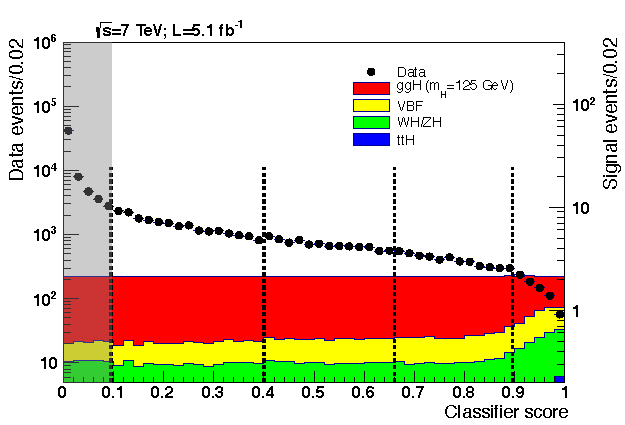
\includegraphics[width=0.475\textwidth]{selec_and_cats/plots/mixedbdt_transformed_7TeV_fix_fix.pdf} \hspace{0.05cm}
  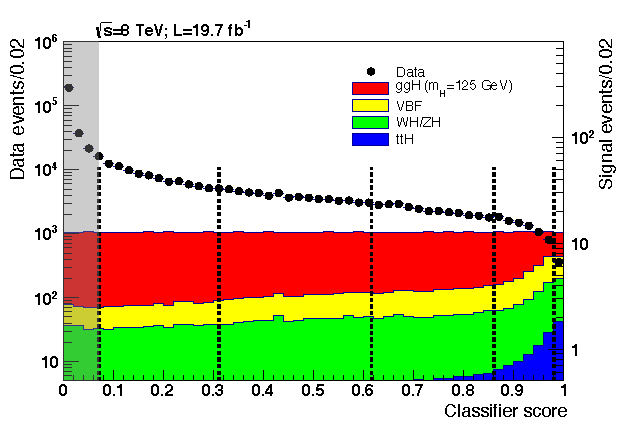
\includegraphics[width=0.475\textwidth]{selec_and_cats/plots/mixedbdt_transformed_8TeV_fix_fix.pdf} \\ 
  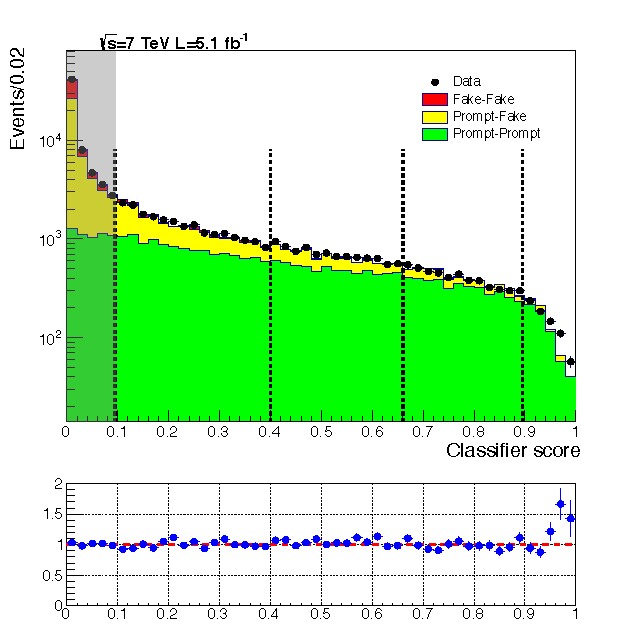
\includegraphics[width=0.48\textwidth]{selec_and_cats/plots/diphobdt_transformed_bg_7TeV_fix_fix.pdf} \hspace{0.05cm}
  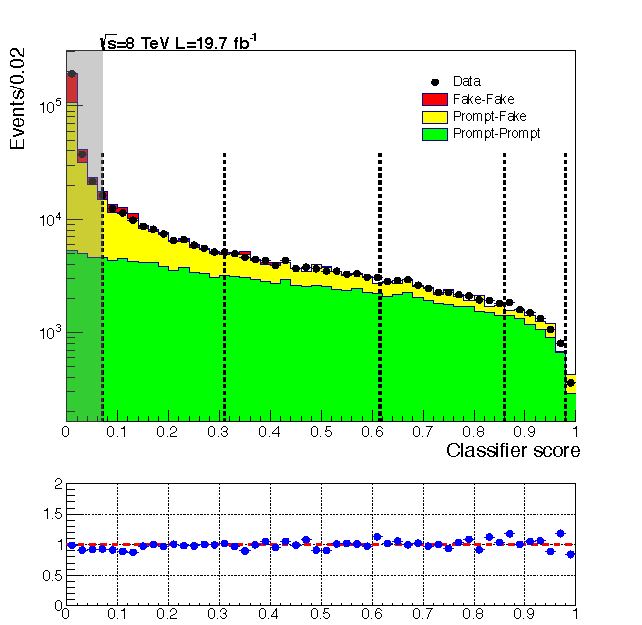
\includegraphics[width=0.48\textwidth]{selec_and_cats/plots/diphobdt_transformed_bg_8TeV_fix_fix.pdf}
  \caption[The diphoton \acs{BDT} response]{The diphoton \BDT response for the 7~\TeV training (left column) and 8~\TeV training (right column) transformed so that the output is flat in the signal. The top row shows the output in data (black points), which contains mostly background events, and signal \MC events (filled histograms) split by production mode; \ggH (red), \VBF (yellow), \VH (green), \ttH (blue). The bottom row shows the output in data (black points) and background \MC events (filled histograms) split by type; prompt-prompt (green), prompt-fake (yellow) and fake-fake (red). The data/background residual is shown as the blue points underneath these histograms. The vertical dashed lines show the analysis category definitions where those on the right (nearer a classifier score of 1) have the highest S/B ratio. All events which fall below the left most boundary, shown by the shaded area, are cut out of the analysis.}
  \label{fig:dipho_bdt}
\end{figure}

Any uncertainties which affect the shape of the output distribution of this \BDT result in event migrations between the final analysis categories; if the \BDT response is mismodelled then events can move across the boundaries represented as the vertical dashed lines in Fig.~\ref{fig:dipho_bdt}. The signal model in this analysis is obtained from \MC simulation and so these uncertainties can have an effect on the signal model shape in each of the categories. Whilst these migrations may also be true of the background the effect is not important because the background is extracted from data. The input variables whose uncertainties have the largest effect on the \BDT response in signal are the photon ID quality and the photon energy resolution estimate. This is because these variables have both i) relatively large uncertainties because of imperfect detector response modelling in the simulation and ii) are highly discriminative and hence can have a relatively large impact on the \BDT response. As the \BDT response varies monotonically with these variables, the sytematic uncertainty on them is propagated through the analysis as an event migration. Systematic uncertainties are described in more detail in Sec.~\ref{sec:systematics}. The size of this effect is shown in the \BDT response validation plot using the \Zee decay in Fig.~\ref{fig:diphotonBDT_zee}.

\begin{figure}
  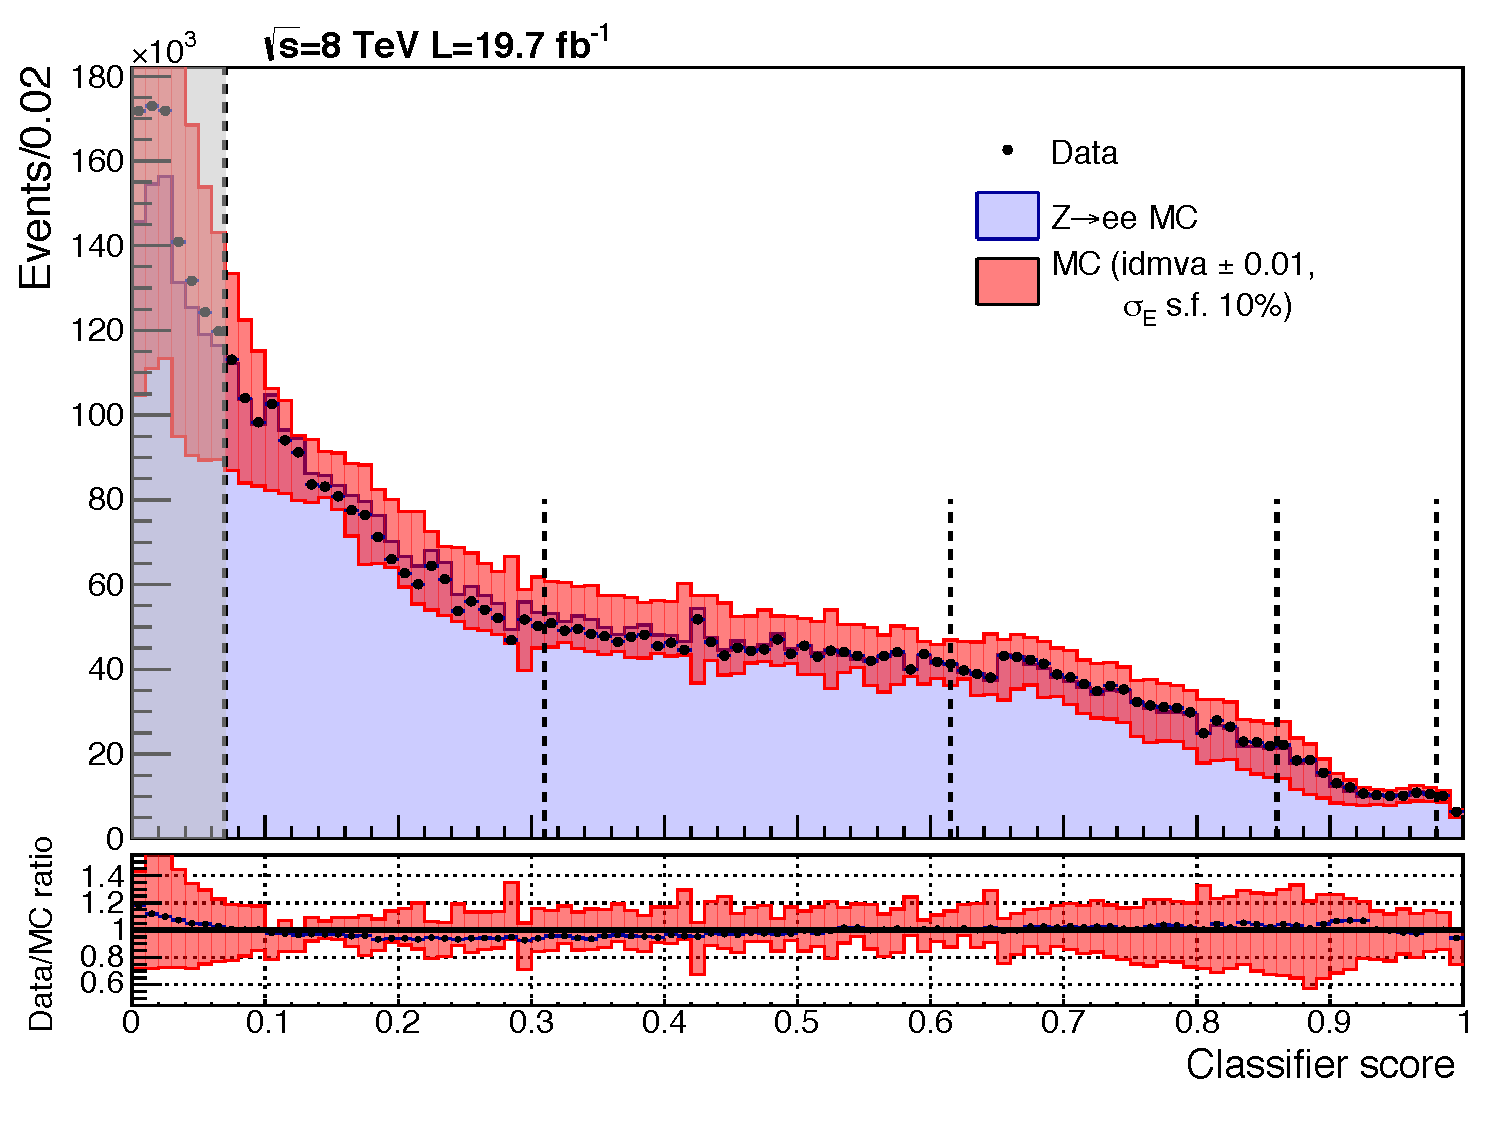
\includegraphics[width=0.95\textwidth]{selec_and_cats/plots/transformedBDT_single_syst_fix_fix.pdf}
  \caption[The diphoton \acs{BDT} response in \Zee decays]{The diphoton BDT response for the 8~\TeV training in the \Zee decay. The data is shown as the black points and the \MC events as the blue histogram. The systematic applied to account for variation in the BDT response from mismodelling in the photon quality response and the photon energy resolution estimate are shown as the red band. The vertical dashed lines show the boundaries of the analysis categories.}
  \label{fig:diphotonBDT_zee}
\end{figure}

% ---- SECTION ----
\section{Event categorisation}
\label{sec:categorisation}

In order to exploit different regions of phase space with dissimilar signal to background ratios the events are split into categories. Furthermore, additional categories can be designed to enrich the selection with events characteristic of particular Higgs production modes. The \VBF production mode is typically accompanied by a pair of jets with a large pseudorapidity separation, the \VH production, which includes contributions from \WH and \ZH, may be accompanied by a charged lepton, missing transverse energy or jets originating from the decay of the associated $W$ or $Z$ boson. Similarly, \ttH production may be accompanied by $b$ quarks and/or charged leptons. The predominant production mode, which accounts for about 88\% of the signal, is \ggH which is inclusive. The amount of signal produced from exclusive modes is approximately 8\% for \VBF, 4\% for \VH and $<$1\% for \ttH. By including a series of event tags, and separating events accordingly, all four production modes of the Higgs at the \LHC are harnessed in this analysis. This not only helps to increase the overall sensitivity to a \SM Higgs boson (given the very low background rates expected for the exclusive modes) but also significantly helps to reduce the error on measurements of the relative couplings of the observed boson to fermions and bosons, as the signal from the relative production modes gets split into distinct categories. This ``exclusive mode tagging" is done identically for both the nominal \MFM analysis and also the cross check \SMVA, although the inclusive mode categorisation is done differently. The \CiC spin analysis uses no exclusive mode tagging as the spin-2 models considered (minimal coupling graviton) have only inclusive production modes. There is an alternate categorisation scheme used for the spin analysis which exploits both the event mass resolution and the differential decay angle. 

\subsection{Exclusive mode tagging}
\label{sec:exclusive_tags}
All events which make it to this stage will have passed the photon preselection (Sec.~\ref{sec:photon_presel}), as well as the basic requirement of two high \pT photons with $100<m_{\gamma\gamma}<180$~GeV (Sec.~\ref{sec:event_selection}) and the MVA selection (Sec.~\ref{sec:diphoton_bdt}) and these make up the final event sample. They now pass through the ``tagging" procedure described below in which they are organised into a set of non-overlapping event classes. The tagging is done in a specific order to ensure there is no overlap between classes and the order is chosen such that preference is given to categories with a higher expected signal to background ratio. This order is shown alongside a summary of the relevant cut values in Table~\ref{tab:cat_summary} at the end of the chapter. If an event does not meet the requirements of a particular tag it is passed onto the next tag and if it fails all tag requirements it is placed in one of the inclusive categories, whose structure is described below (Secs.~\ref{sec:inclusive_cats_massfac}-\ref{sec:inclusive_cats_sideband}), meaning that no event cannot be included in the analysis. 

\subsubsection{Dijet tagged categories for VBF}
\label{sec:vbf_tag}

The following variables are used to exploit the specific topolgy of the jet pairs associated to \VBF Higgs production:

\begin{itemize}
  \item $p_{T}^{\gamma}/m_{\gamma\gamma}$ - The transverse momenta of the leading and subleading photons as a ratio of the diphoton invariant mass.
  \item $p_{T}^{\mathrm{j}}/m_{\gamma\gamma}$ - The transverse momenta of the leading and subleading jets as a ratio of the diphoton invariant mass.
  \item $m_{\mathrm{jj}}$ - The dijet invariant mass.
  \item $|\Delta\eta_{\mathrm{j}_{1}\mathrm{j}_{2}}|$ - The absolute pseudorapidity difference between the two jets.
  \item $Z = \eta(\gamma_{1})+\eta(\gamma_{2}) - \bigl[\eta(\mathrm{j}_{1})+\eta(\mathrm{j}_{2})\bigr]/2$ - The so-called \emph{Zeppenfeld} variable~\cite{Zeppenfeld}.
  \item $\Delta\phi_{\mathrm{j}_{1}\mathrm{j}_{2}}$ - The angular difference between the two jets in the transverse plane.
\end{itemize}

Additionally the leading photon \pT requirement is raised to $p_{T}^{\gamma_{1}}/m_{\gamma\gamma}>1/2$. The energy measurement of jets in the event are calibrated to correct for detector effects~\cite{jet_energy_corrections} and additional energy in the jets from pileup is removed using the \textsc{FastJet} jet areas technique described in~\cite{pu_jets1,pu_jets2,pu_jets3}. Jets are required to be within the pseudorapidity range $|\eta|<4.7$.

The dijet tagging is done with use of two additional \MVAs. The first is designed to exploit the \VBF kinematic properties and the second is used to combine this information with the diphoton \BDT. Candidates are required to pass a \VBF preselection of two jets with $p_{T}^{\j_{1}}>30$~\GeV and $p_{T}^{\j_{2}}>20$~\GeV and invariant mass, \mjj$>75$~\GeV. The signal sample used for training is the \SM \MC simulation with just \VBF production, whilst the \SM gluon fusion \MC simulation is included as background along with the usual prompt-prompt, prompt-fake and fake-fake contributions. This helps produce an output in which a high score gives a very pure \VBF sample.

The combined dijet-diphoton \BDT has inputs of the kinematic dijet \BDT output, the diphoton \BDT output and $p_{T}^{\gamma\gamma}/m_{\gamma\gamma}$ in order to discriminate \VBF from both the other signal types and the background, utilising all the information available in the event. The transverse momenta of the diphoton system as a ratio of the diphoton invariant mass, $p_{T}^{\gamma\gamma}/m_{\gamma\gamma}$, is included both because of its discriminatory power and its considerable correlation with both the dijet \BDT output and the diphoton \BDT output.

One finds that the background rejection for \VBF is significantly improved by the use of the combined dijet-diphoton \BDT whilst the \VBF purity (i.e.~separation from \ggH) is not as good when collapsing the kinematic dijet \BDT and the combined \BDT into one step. Consequently the trainings are performed separately and the \VBF categories are defined by picking out regions which have a high score in the combined dijet-diphoton \BDT response. Each successive \BDT training uses statisically independent \MC samples to avoid selection bias from fluctuations in the simulation. The optimisation procedure for deciding the category boundaries is analogous to the one used for the inclusive categories in the \MFM analysis where the target is to minimise the expected uncertainty of the signal strength from the \VBF process alone when moving the boundaries around. The optimisation procedure includes the statistical disadvantage of having too many categories for a given dataset size. It is explained further in Section~\ref{sec:inclusive_cats_massfac}. At 8~\TeV there are three \VBF categories and at 7~\TeV there are two, because of the considerably lower statistics in the 7~TeV dataset. The output distributions at 7 and 8~TeV for the signal and the data are shown for the kinematic dijet \BDT in Fig.~\ref{fig:vbf_dijet_kin} and for the combined diphoton-dijet \BDT, along with the \VBF category boundaries, in Fig.~\ref{fig:vbf_dijet_comb}. The \BDT response shown in these plots is transformed so that it is flat in the \VBF signal (yellow histogram). One can see that the other signal types peak lower in the transformed score and the data, which contains mostly background, even more so. 

\begin{figure}
  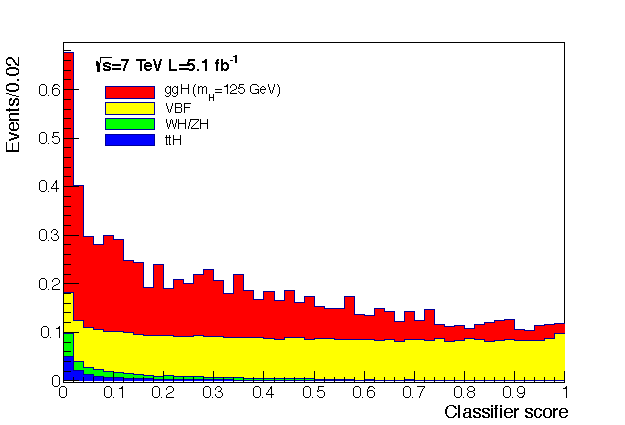
\includegraphics[width=0.48\textwidth]{selec_and_cats/plots/dijetbdt_transformed_signal_7TeV_fix_fix.pdf}
  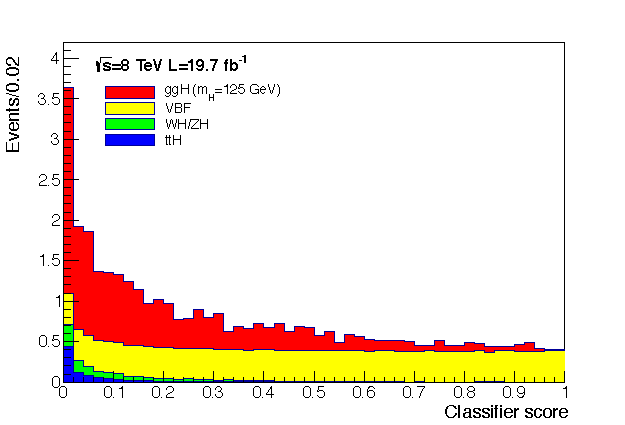
\includegraphics[width=0.48\textwidth]{selec_and_cats/plots/dijetbdt_transformed_signal_8TeV_fix_fix.pdf} 
  \caption[The kinematic dijet \acs{BDT} response]{The distributions of the kinematic dijet \BDT response at 7~TeV (left) and 8~TeV (right) for the signal split by production mode; \ggH (red), \VBF (yellow), \VH (green) and \ttH (blue). The output is transformed so that it is flat in the \VBF signal.}
  \label{fig:vbf_dijet_kin}
\end{figure}

\begin{figure}
  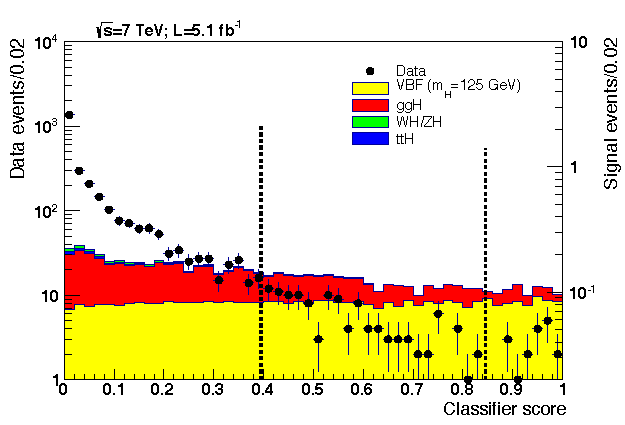
\includegraphics[width=0.48\textwidth]{selec_and_cats/plots/mixedcombbdt_transformed_7TeV_fix_fix.pdf}
  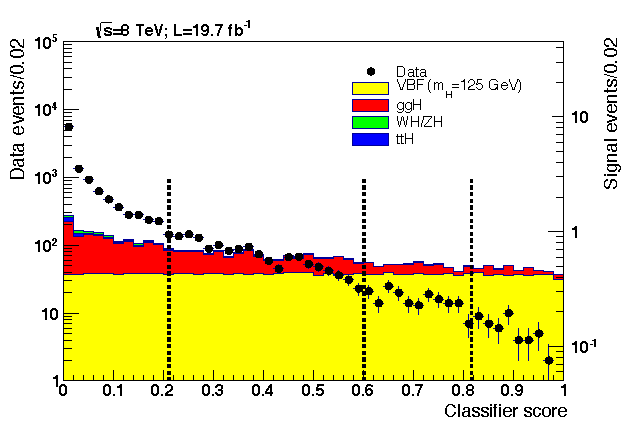
\includegraphics[width=0.48\textwidth]{selec_and_cats/plots/mixedcombbdt_transformed_8TeV_fix_fix.pdf}
  \caption[The distribution of the combined dijet-diphoton \acs{BDT} response]{The distributions of the combined dijet-diphoton \BDT response at 7~TeV (left) and 8~TeV (right) for the data (black points), which contains mostly background, and signal (filled histograms) split by production mode; \ggH (red), \VBF (yellow), \VH (green) and \ttH (blue). The output is transformed so that it is flat in the \VBF signal. The vertical dashed lines show the \VBF category definitions where those on the right (nearer a classifier score of 1) are purest \VBF signal. All events which fall below the left most boundary are not included in \VBF categories but fall back to being categorised amongst the inclusive categories.}
  \label{fig:vbf_dijet_comb}
\end{figure}

\subsubsection{Lepton, jet and \MET tagged categories for \VH}
\label{sec:vh_tag}

The selection for the four categories designed to tag \VH production are optimised by minimising the expected uncertainty on the signal strength of this process alone. Two of the classes require at least one charged muon or electron and are split into a tight selection category and a looser selection category, the third is for events consistent with large \MET and the fourth for events consistent with two or more jets. The leading photon cut is raised to $p_{T}^{\gamma_{1}}/m_{\gamma\gamma}>3/8$ for all \VH-tagged categories. The category requirements are as follows,

\begin{itemize}
  \item \textbf{\VH Tight $l$}: The tighly selected lepton category is characterised by the signature of a leptonically decaying $W$ or $Z$ boson and as such requires the presence of \MET$>35$~\GeV or another lepton of the same flavour and opposite charge as the first. In the first case (of a lepton + \MET) the lepton is required to have $p_{T}>20$~\GeV, in the latter case (of two leptons) the requirement is $p_{T}>10$~\GeV for both leptons whilst the invariant mass of the dilepton pair must be $70 < m_{ll} < 110$~\GeV. The diphoton \BDT output is required to be $>0.1$ ($>-0.6$) for the 7 (8)~\TeV datasets.
  \item \textbf{\VH Loose $l$}: For the loosely selected lepton category the lepton \pT must satisfy $p_{T}>20$~\GeV. The selection requirements are designed to reduce the background from leptonic $Z$ bosons (not associated with a Higgs) that contain initial or final state radiation faking the diphoton signal. Consequently, leptons are required to be separated by at least $\Delta R>1.0$ from the closest photon and the invariant mass of any lepton-photon pairs must be more than 10~\GeV away from the $Z$ boson mass. In addition a conversion veto is applied to the electrons to reduce the rate of misidentified photons. The diphoton \BDT output is required to be $>0.1$ ($>-0.6$) for the 7 (8)~\TeV datasets.
  \item \textbf{\VH \MET tag}: Accurate measurement and simulation of the \MET vector has been studied in detail at \CMS and a set of standard corrections (for both data and simulation) are applied~\cite{met_corrs}. The corrected \MET is required to pass \MET$>70$~\GeV whilst the angular separation in the transverse plane betwen the momentum of the diphoton system and the \MET direction must pass $\Delta\phi(\gamma\gamma,\MET)>2.1$, and similarly the angle between the momentum of the diphoton system and the leading jet must pass $\Delta\phi(\gamma\gamma,\mbox{jet})<2.7$. The diphoton \BDT output is required to be $>0.8$ ($>0.0$) for the 7 (8)~\TeV datasets.   
  \item \textbf{\VH dijet tag}: The event must contain at least one jet pair in which both jets have $p_{T}>40$~\GeV and $|\eta|<2.4$ and have an invariant mass within the range $60<m_{jj}<120$~\GeV. The diphoton transverse momentum must satisfy $p_{T}^{\gamma\gamma}/m_{\gamma\gamma}>13/12$. Additionally the angular correlation between the diphoton system and the dijet system from \VH-associated Higgs decays can be exploited. The angle, $\theta^{\star}$, between the diphoton direction in the diphoton-dijet rest frame and the lab frame is flat for events from \VH decays whereas for the background and gluon fusion-produced Higgs decays the distribution peaks at $|\cos(\theta^{\star})|=1$. Consequently, there is a requirement that $|\cos(\theta^{\star})|<0.5$. The diphoton \BDT output is required to be $>0.6$ ($>0.2$) for the 7 (8)~\TeV datasets. 
\end{itemize}

\subsubsection{Lepton and jet tagged categories for \ttH}
\label{sec:tth_tag}

There are two categories for tagging production from \ttH decays, one of which is lepton-based and one of which is jet-based. The total fraction of signal expected from \ttH is $<$1\% so only a handful of events are expected. Consequently for the 7~\TeV dataset the two categories are merged into one class. As for the \VH-tagged categories, the cuts are optimised to minimise the expected uncertainty of the signal strength measurement of the \ttH process alone.

For both classes the leading photon \pT cut is raised to $p_{T}^{\gamma_{1}}/m_{\gamma\gamma}>1/2$, all jets are required to have \pT$>25$~\GeV and there must be at least one b-tagged jet present. The specific requirements of each category are as follows,

\begin{itemize}
  \item \textbf{\ttH multijet tag}: The requirement is at least four additional jets in the event and no lepton. The diphoton \BDT output is required to be $>0.6$ ($>-0.2$) for the 7 (8)~\TeV datasets. 
  \item \textbf{\ttH lepton tag}: At least one more jet in the event and one muon or electron which has \pT$>20$~\GeV. The diphoton \BDT output is required to be $>0.6$ ($>-0.6$) for the 7 (8)~\TeV datasets.  
\end{itemize}

%\subsection{Inclusive mode categorisation in the cut based analysis}
%\label{sec:inclusive_cats_cic}

%Any event which passes the cut based photon selection described in Section~\ref{sec:cic} and does not fall into one of the exclusive categories described above is split into one of eight inclusive categories depending on the supercluster position, \eta, of the two photons, the conversion variable, \rnine, of the two photons and the mass relative diphoton transverse momenta, \pToM. The categories are defined in Table~\ref{tab:cic_cats}.

%\begin{table}
%  \begin{center}
%    \begin{tabular}{lccc}
%                 & \pToM                            & Maximum \eta                                    & Minimum \rnine \\
%      \hline
%      Untagged 0 & \multirow{4}{*}{$>40$~\GeV}      & \multirow{2}{*}{$<$1.444}                       & $>0.94$ \\
%      Untagged 1 &                                  &                                                 & $<0.94$ \\
%      Untagged 2 &                                  & \multirow{2}{*}{$<$2.5}                         & $>0.94$ \\
%      Untagged 3 &                                  &                                                 & $<0.94$ \\
%      \hline
%      Untagged 4 & \multirow{4}{*}{$<40$~\GeV}      & \multirow{2}{*}{$<$1.444}                       & $>0.94$ \\
%      Untagged 5 &                                  &                                                 & $<0.94$ \\
%      Untagged 6 &                                  & \multirow{2}{*}{$<$2.5}                         & $>0.94$ \\ 
%      Untagged 7 &                                  &                                                 & $<0.94$ \\
%    \end{tabular}
%    \caption{The definition of the inclusive categories for the \CiC analysis}
%    \label{tab:cic_cats}
%  \end{center}
%\end{table}

\subsection{Inclusive mode categorisation and VBF dijet categorisation in the mass factorised \MVA analysis}
\label{sec:inclusive_cats_massfac}

The combined dijet-diphoton \BDT output value is used to define a set of \VBF categories. The goal is to find the configuration of category boundaries which minimise the expected uncertainty on the signal strength for \VBF production alone, allowing the number of categories and where the category boundaries lie to be completely free floating, with the additional requirement that the efficiency $\times$ acceptance of the categories matches between 7 and 8~\TeV. This results in a tight \VBF category for events with a very high combined dijet-diphoton \BDT score, a somewhat looser category and then one or more very loose categories. It is found that dropping the loosest category has a negligible impact ($<$1\%) on the expected uncertainty and as such the upper boundary for the loosest category is turned into a lower cut. All events which pass the \VBF preselection (described in Sec.~\ref{sec:vbf_tag}) and fail the lower cut are then classified somewhere in the inclusive categories defined below. 

Once the \VBF category boundaries have been found the same procedure is deployed using the diphoton \BDT output value. This time the target is to minimise the expected uncertainty on the total signal strength, allowing the number of categories and the category boundary values to be completely free floating. One finds a rather similar structure and that dropping events in the very loosest category has a neglible impact on the performance and consequently this dictates the lower cut value for the diphoton \BDT. The expected uncertainty minima, when floating both the number of category boundaries and the boundary locations, are fairly shallow so the exact position of the boundaries has a very small impact on the performance of the analysis. For the 7 (8)~\TeV datasets there are 4 (5) inclusive categories with a lower diphoton \BDT cut of 0.19 ($-0.78$) and 2 (3) \VBF categories\footnote{There are fewer categories in the 7~TeV dataset because there are less statistics}.

\subsection{Inclusive mode categorisation in the sideband \MVA analysis}
\label{sec:inclusive_cats_sideband}

In the \SMVA analysis all the exclusive categories are identical to the \MFM analysis (including the \VBF categories). However the inclusive categorisation is done slightly differently. In the sideband analysis the signal region is defined in a $\pm2$\% window around the hypothesis Higgs mass. The analysis is performed as a cut and count in the signal window over several bins. There is one bin for each exclusive category and then several more for the inclusive. The binning scheme for the inclusive events is defined as follows,

\begin{itemize}
  \item Make two dimensional distributions of the diphoton \BDT score and the distance of the invariant mass from the hypothesised Higgs mass, $\Delta m/m_{H}$, in the $\pm2$\% window for signal and background, as shown in Figure~\ref{fig:sideband_inputs}, where,
    \begin{equation}
      \frac{\Delta m}{m_{H}} = \frac{m_{\gamma\gamma} - m_{H}}{m_{H}}.
    \end{equation}
  \item Use a local regression smoothing technique~\cite{regression_smoothing} to smooth statistical fluctutations within the sample (demonstrated in Fig.~\ref{fig:sideband_inputs}).
  \item Select bins by isolating regions of this 2D phase space which have similar $S/B$ ratios and optimise the boundaries to give the maximum expected signal significance.   
\end{itemize}

Clearly the most sensitive bins will be the ones which have a high diphoton \BDT score and have a low value of $|\dmom|$ (i.e.\ are near the signal peak). The category boundaries in this 2D plane are shown as different shades in Figure~\ref{fig:sideband_cats}. In total there are 8 (10) inclusive bins for the 7 (8)~\TeV samples in the \SMVA.

\begin{figure}
  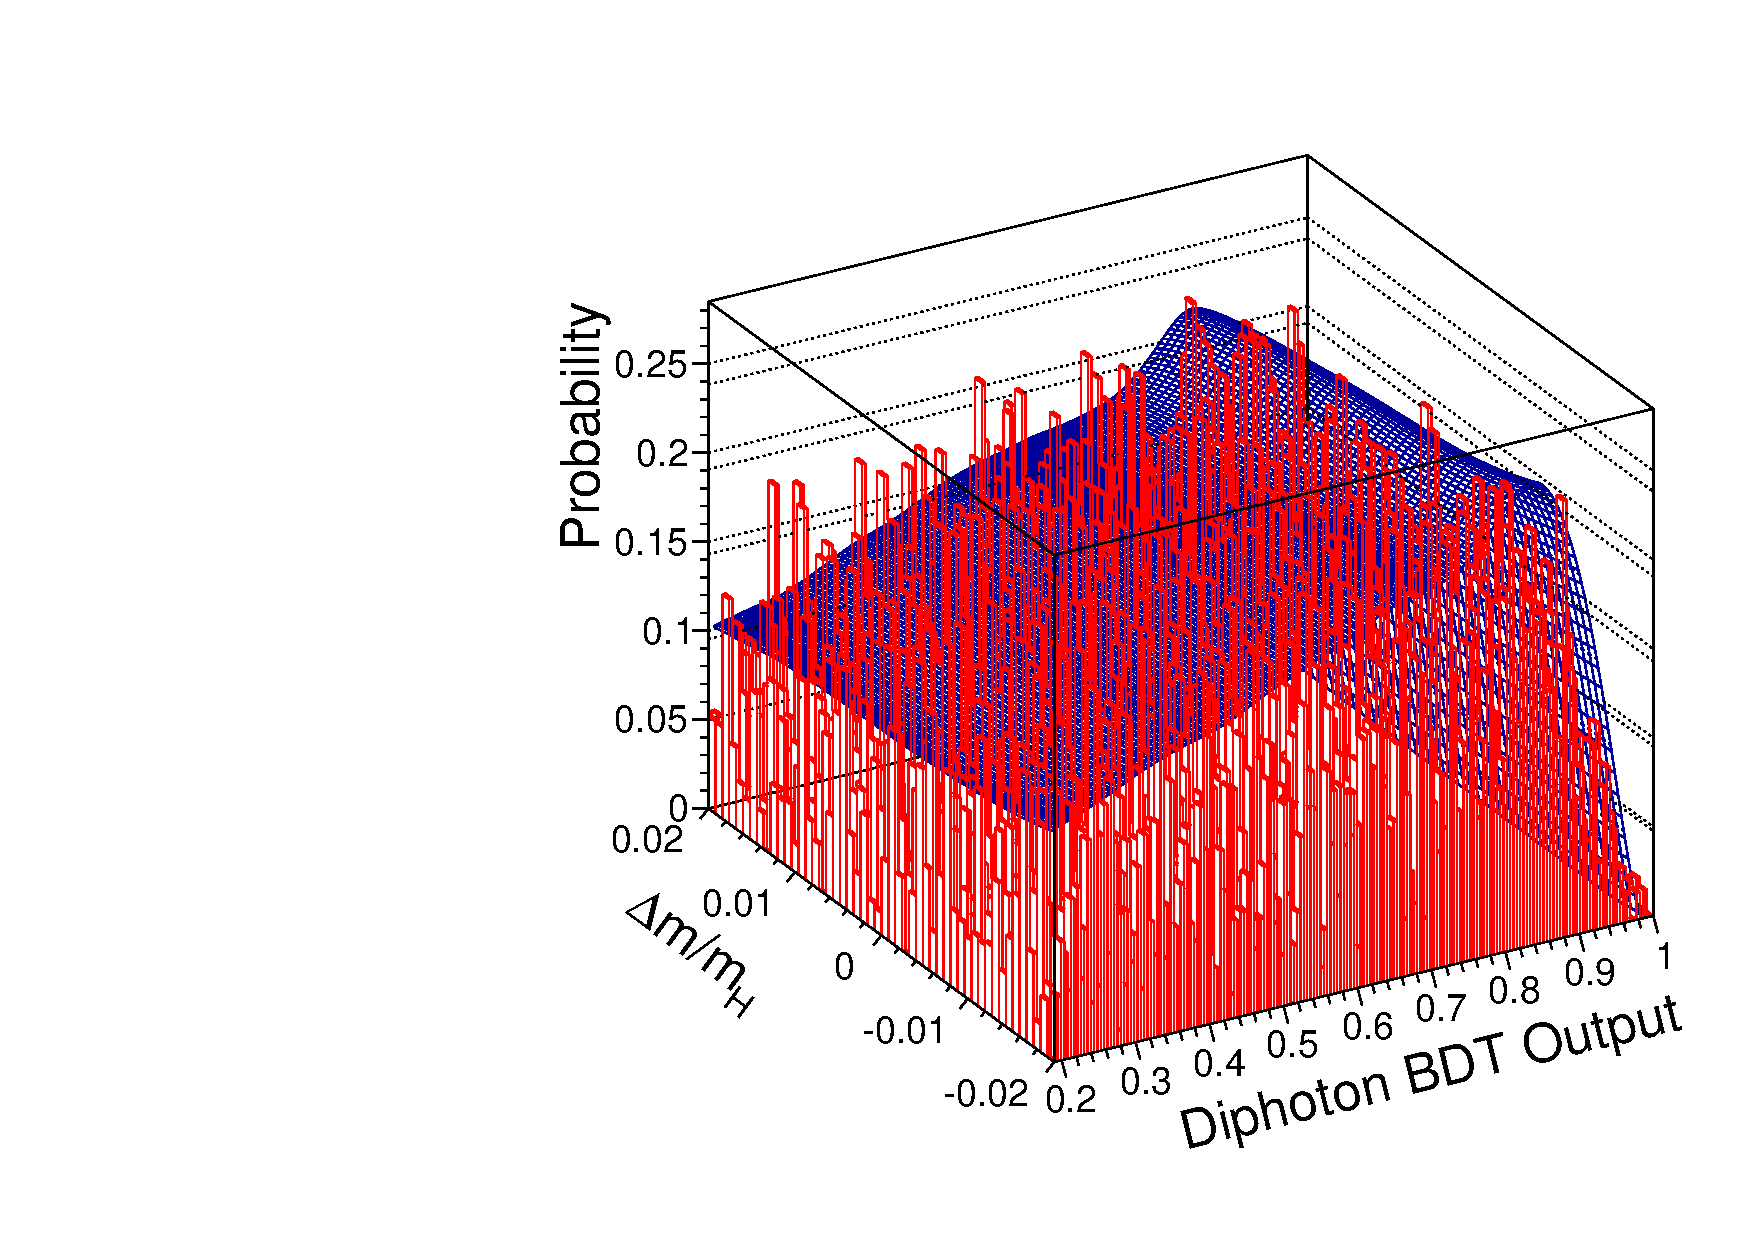
\includegraphics[width=0.48\textwidth]{selec_and_cats/plots/sideband_bkg_7TeV_fix.pdf}
  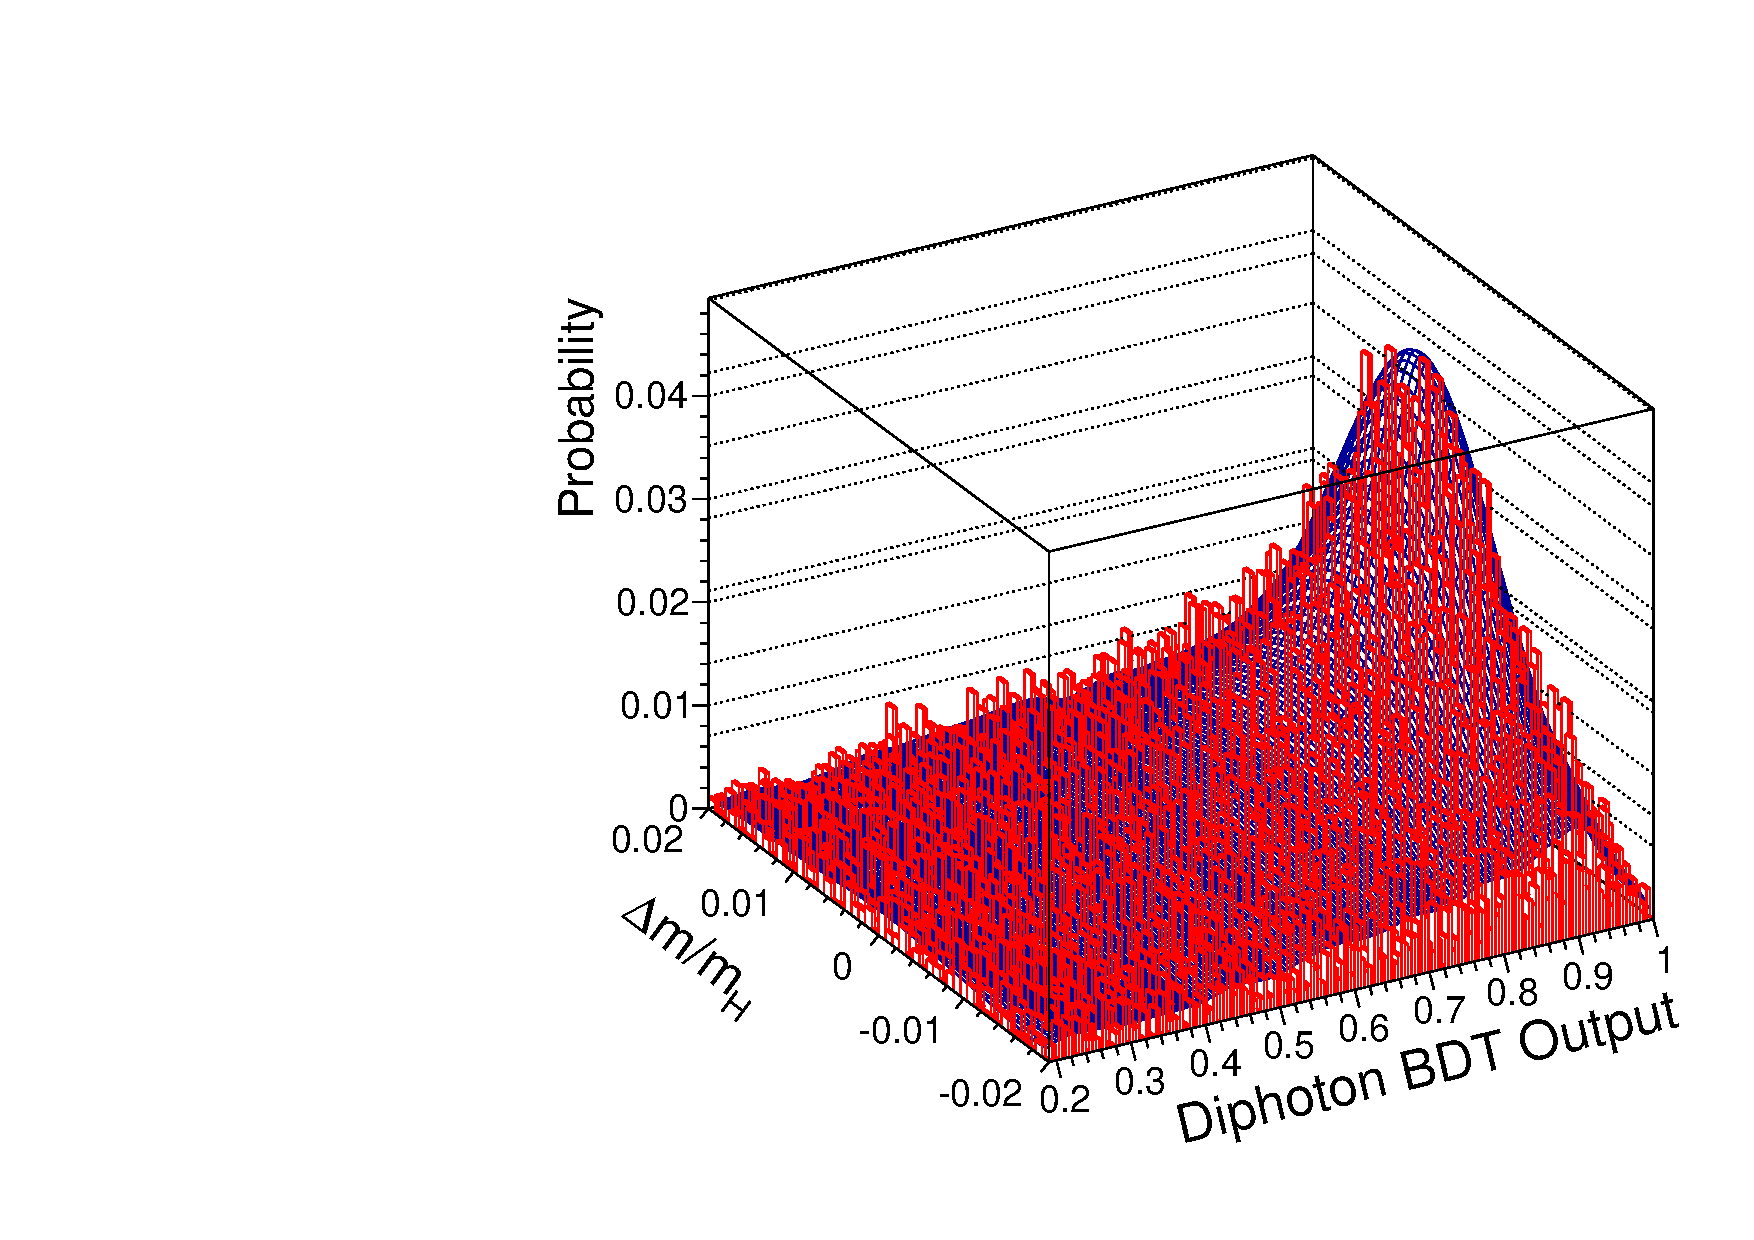
\includegraphics[width=0.48\textwidth]{selec_and_cats/plots/sideband_sig_7TeV_fix.pdf} \\
  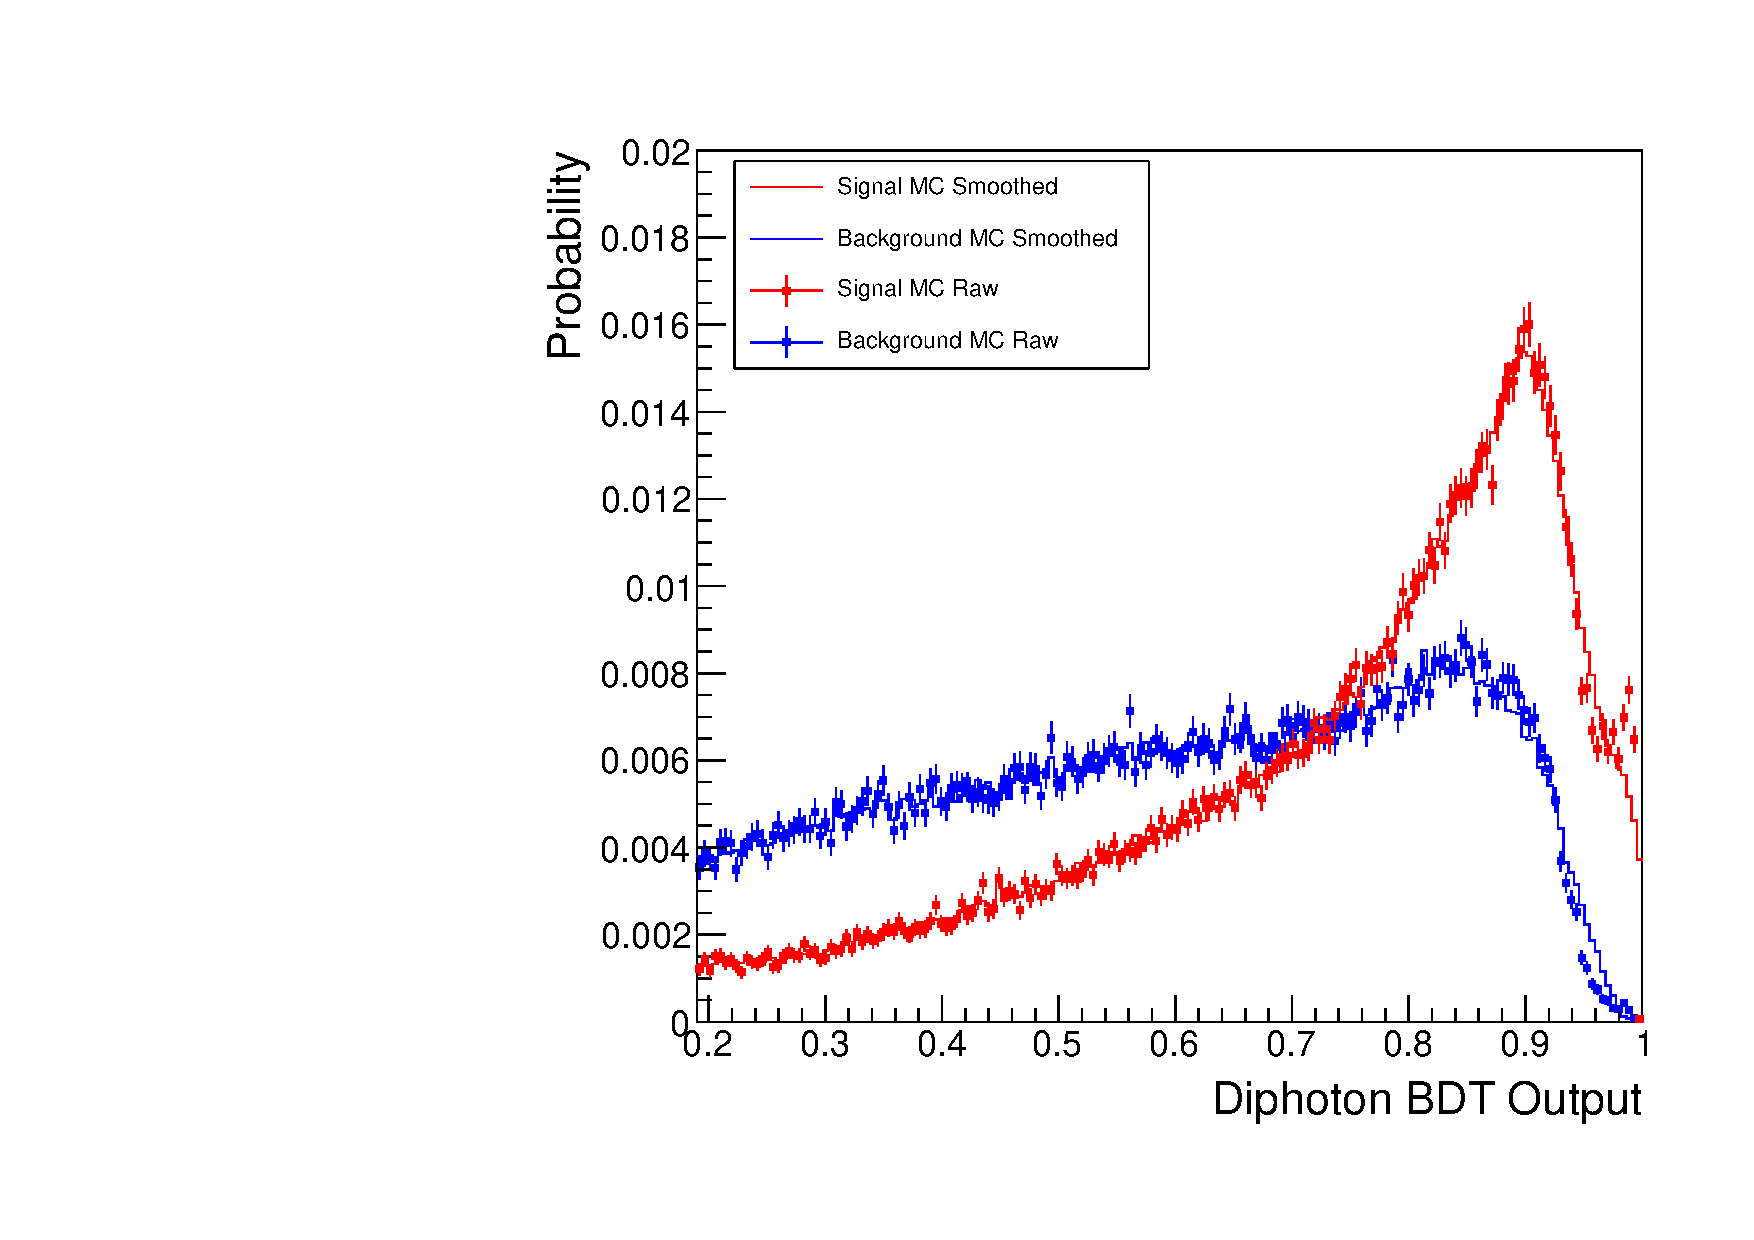
\includegraphics[width=0.48\textwidth]{selec_and_cats/plots/sideband_diphobdt_7TeV_fix.pdf}
  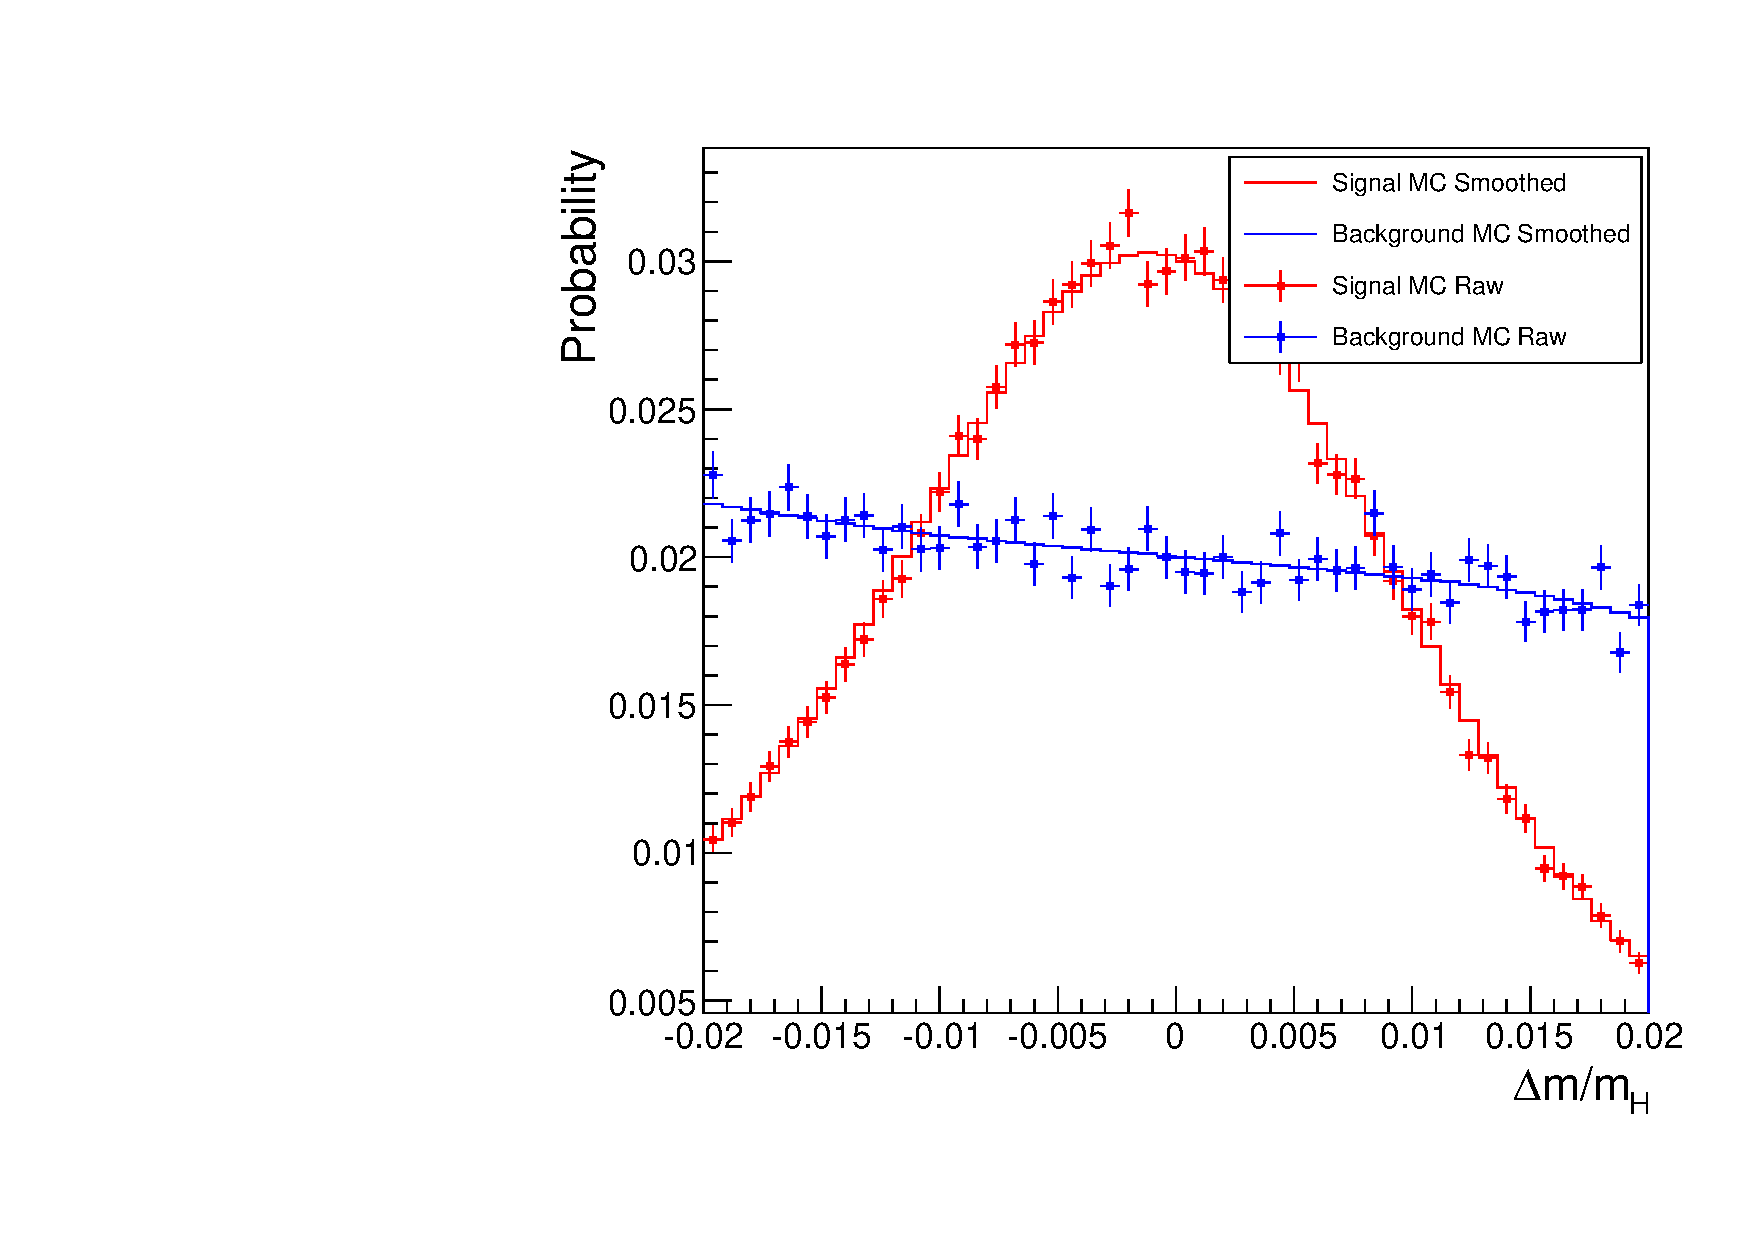
\includegraphics[width=0.48\textwidth]{selec_and_cats/plots/sideband_dmom_7TeV_fix.pdf} \\
  \caption[Two dimensional distributions of the diphoton \acs{BDT} ouput and \dmom for the sideband analysis]{Two dimensional distributions of the diphoton \BDT output and \dmom are shown on the top row for the background (left) and signal (right) for the 7~\TeV sample. The bottom rows show the projection for signal (red) and background (blue) in the two variables.}
  \label{fig:sideband_inputs}
\end{figure}

\begin{figure}
  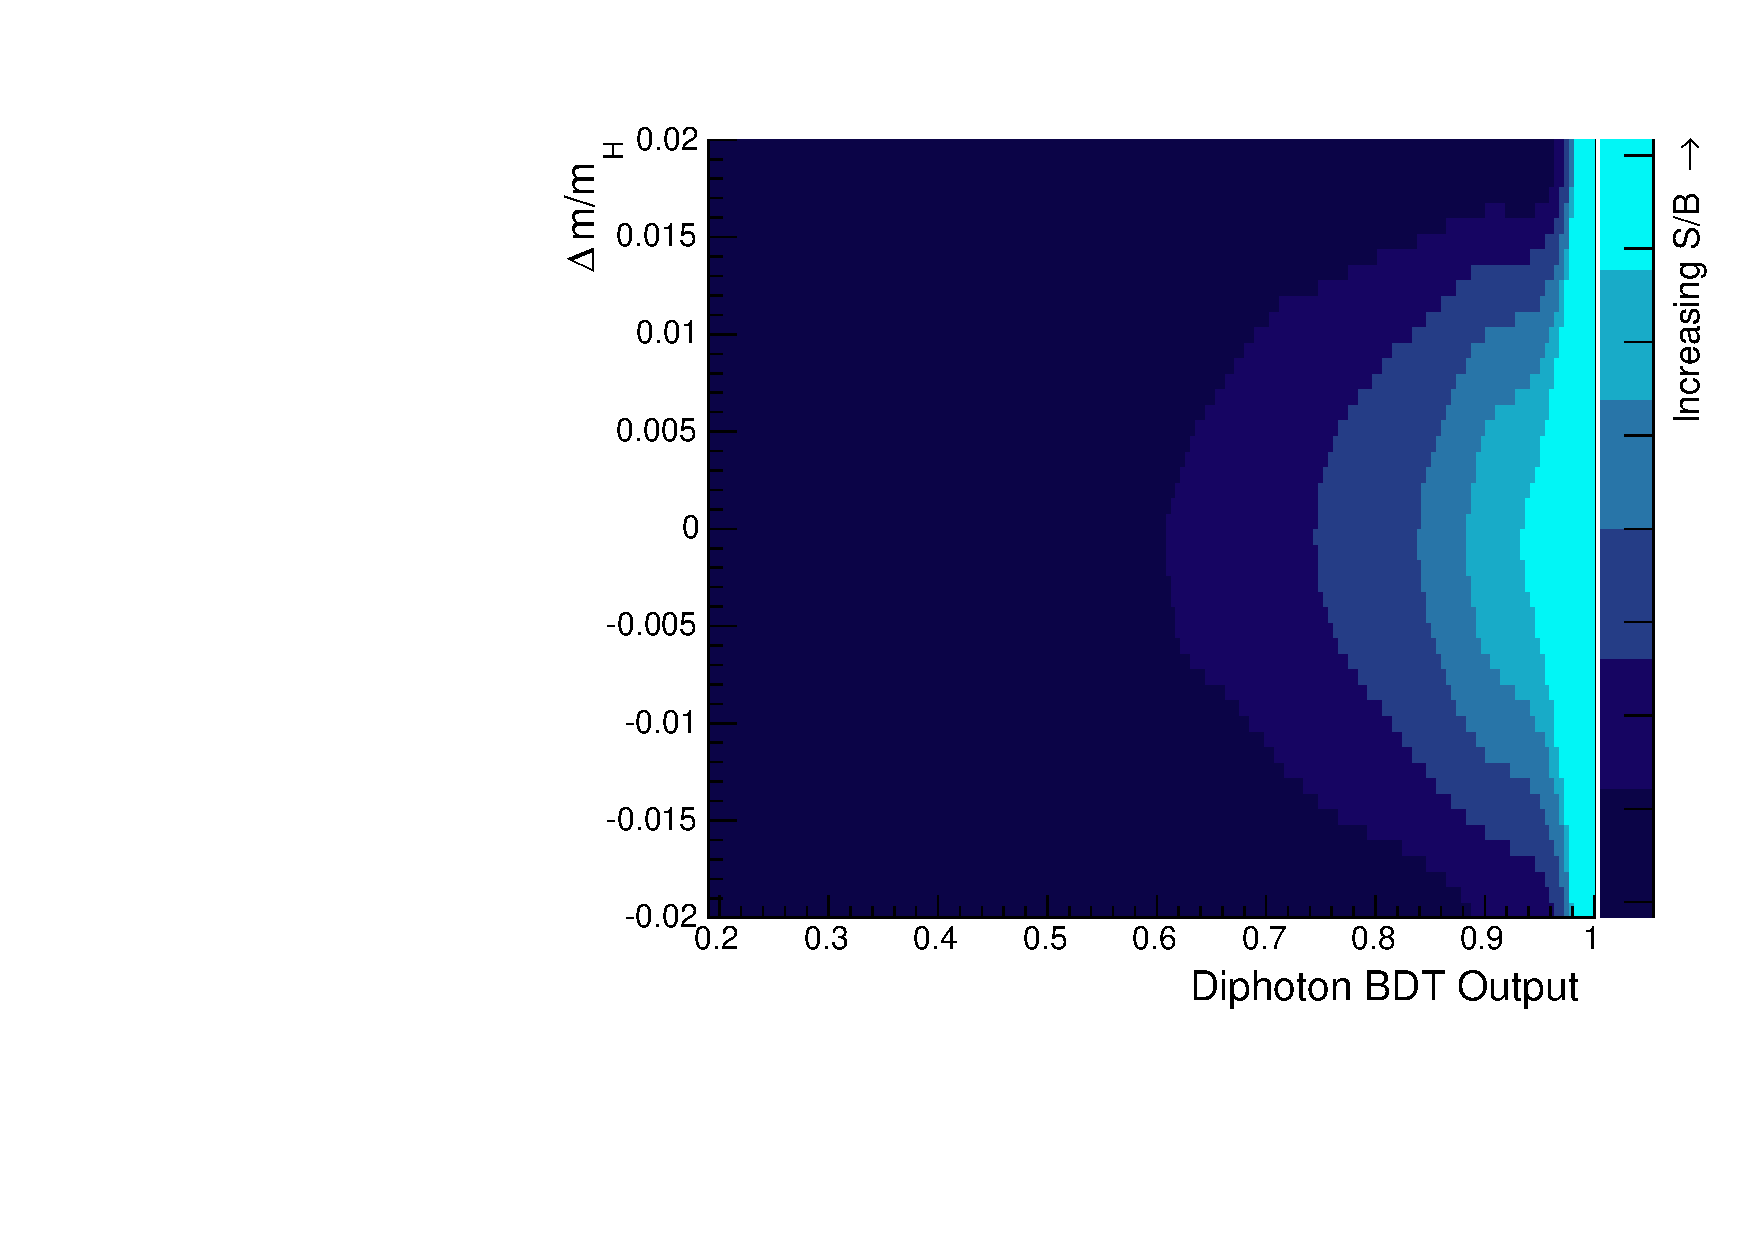
\includegraphics[width=0.48\textwidth]{selec_and_cats/plots/sideband_cats_7TeV_fix.pdf}
  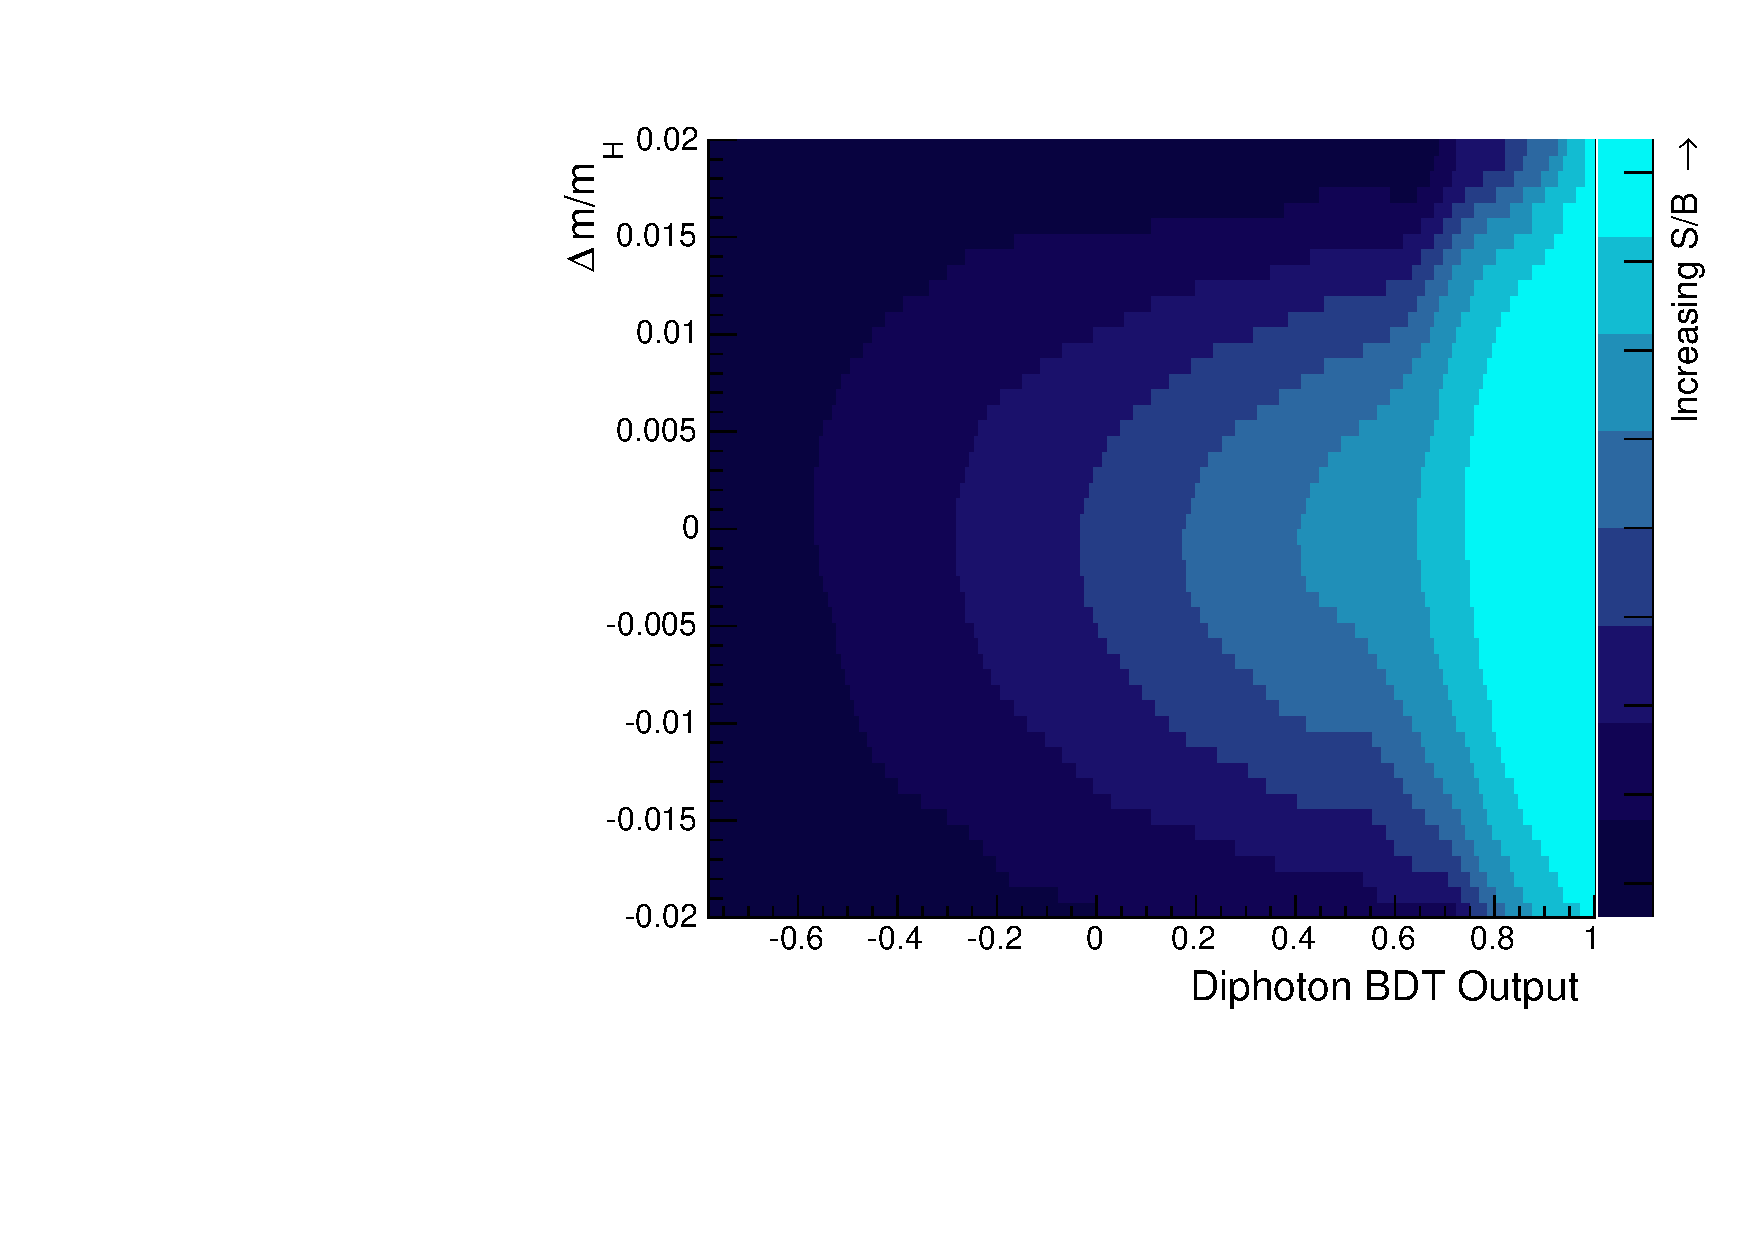
\includegraphics[width=0.48\textwidth]{selec_and_cats/plots/sideband_cats_8TeV_fix.pdf}
  \caption[The inclusive category bin definitions for the \acs{SMVA} analysis]{The inclusive category bin definitions for the \SMVA analysis. Shown for the 7~\TeV dataset on the left and the 8~\TeV dataset on the right.}
  \label{fig:sideband_cats}
\end{figure}

\subsection{Inclusive mode categorisation in the spin analysis}
\label{sec:spin_cats}

The Landau-Yang theorem forbids the direct decay of a spin-1 particle into a pair of photons~\cite{Landau1948,Yang1950}. 
Consequently the spin analysis compares the expectation of the spin-0 SM Higgs, $J^{P}=\zerop$, and the spin-2 \emph{graviton-like} 
model with minimal couplings, \twomp,~\cite{Gao2010}. The \twomp graviton resonance is produced in one of two ways, gluon-fusion ($gg$) 
or quark-antiquark annihilation (\qqbar). As the \twomp is just one of many spin-2 models it is desirable to make the analysis as model independent as possible. As a means of 
discriminating the two hypotheses, use is made of the scattering angle in the Collins-Sopper frame, \costhetastar ~\cite{CollinsSoper1977}, which is defined as the angle, in the diphoton rest frame, between the collinear diphotons 
and the line which bisects one incoming beam with the negative of the other beam, 
\begin{equation}
  \cos(\theta^{\ast}_{\mbox{\tiny{CS}}}) = 2\times\frac{E_{2}p_{z1}-E_{1}p_{z2}}{m_{\gamma\gamma}\sqrt{m^{2}_{\gamma\gamma}+p^{2}_{T\gamma\gamma}}},
  \label{eq:costheta}
\end{equation}
where $E_{1}$ and $E_{2}$ are the energies of the leading and trailing photon, $p_{z1}$ and $p_{z2}$ are the $z$-component momenta 
of the leading and trailing photon and $m_{\gamma\gamma}$ and $p_{T\gamma\gamma}$ are the invariant mass and transerve momenta of the diphoton system.

In its rest frame the photons from the decay of a spin-0 boson are isotropic. Hence prior to acceptance cuts, the distribution of \costhetastar 
under the \zerop hypothesis is uniformly flat. In general this is not the case for spin-2 decays. 

In order to reduce any model dependence in the analysis the cut-based photon selection, described in Sec.~\ref{sec:cic}, is used to pick events. The \MVA methods used for event selection in the nominal analysis use specific \SM \MC training samples and most importantly one of the training variables used, namely $\cos(\phi_{1}-\phi_{2})$, is highly correlated to the angular variable, \costhetastar, which can be used to distinguish spin hypotheses. Furthermore, given the unusual production modes of a spin-2 boson, no exclusive tagging is used in the spin analysis. The impact of using jet variables was studied but it was found that the sensitivity for distinguishing spin hypotheses was improved by a neglible amount.

The effect of the photon selection cuts on the distributions of 
\abscostheta is illustrated in Fig.~\ref{fig:acc_cuts}. Before any acceptance cuts, Fig.~\ref{fig:acc_cuts} (left), the \abscostheta
distribution of the \zerop processes is flat. This is not the case for the \twomp processes (gluon-fusion and quark-antiquark annihilation). After the selection cuts are applied these distributions are considerably distorted, Fig.~\ref{fig:acc_cuts} (right). As a Higgs produced from vector boson-fusion, which is $\sim$8\% of the total (compared to $\sim$88\% from gluon fusion),  is typically produced at higher transverse momentum there is some additional contribution of \zerop signal at high values of \abscostheta compared to the \twomp production modes after the selection cuts.

\begin{figure}
	\begin{center}
	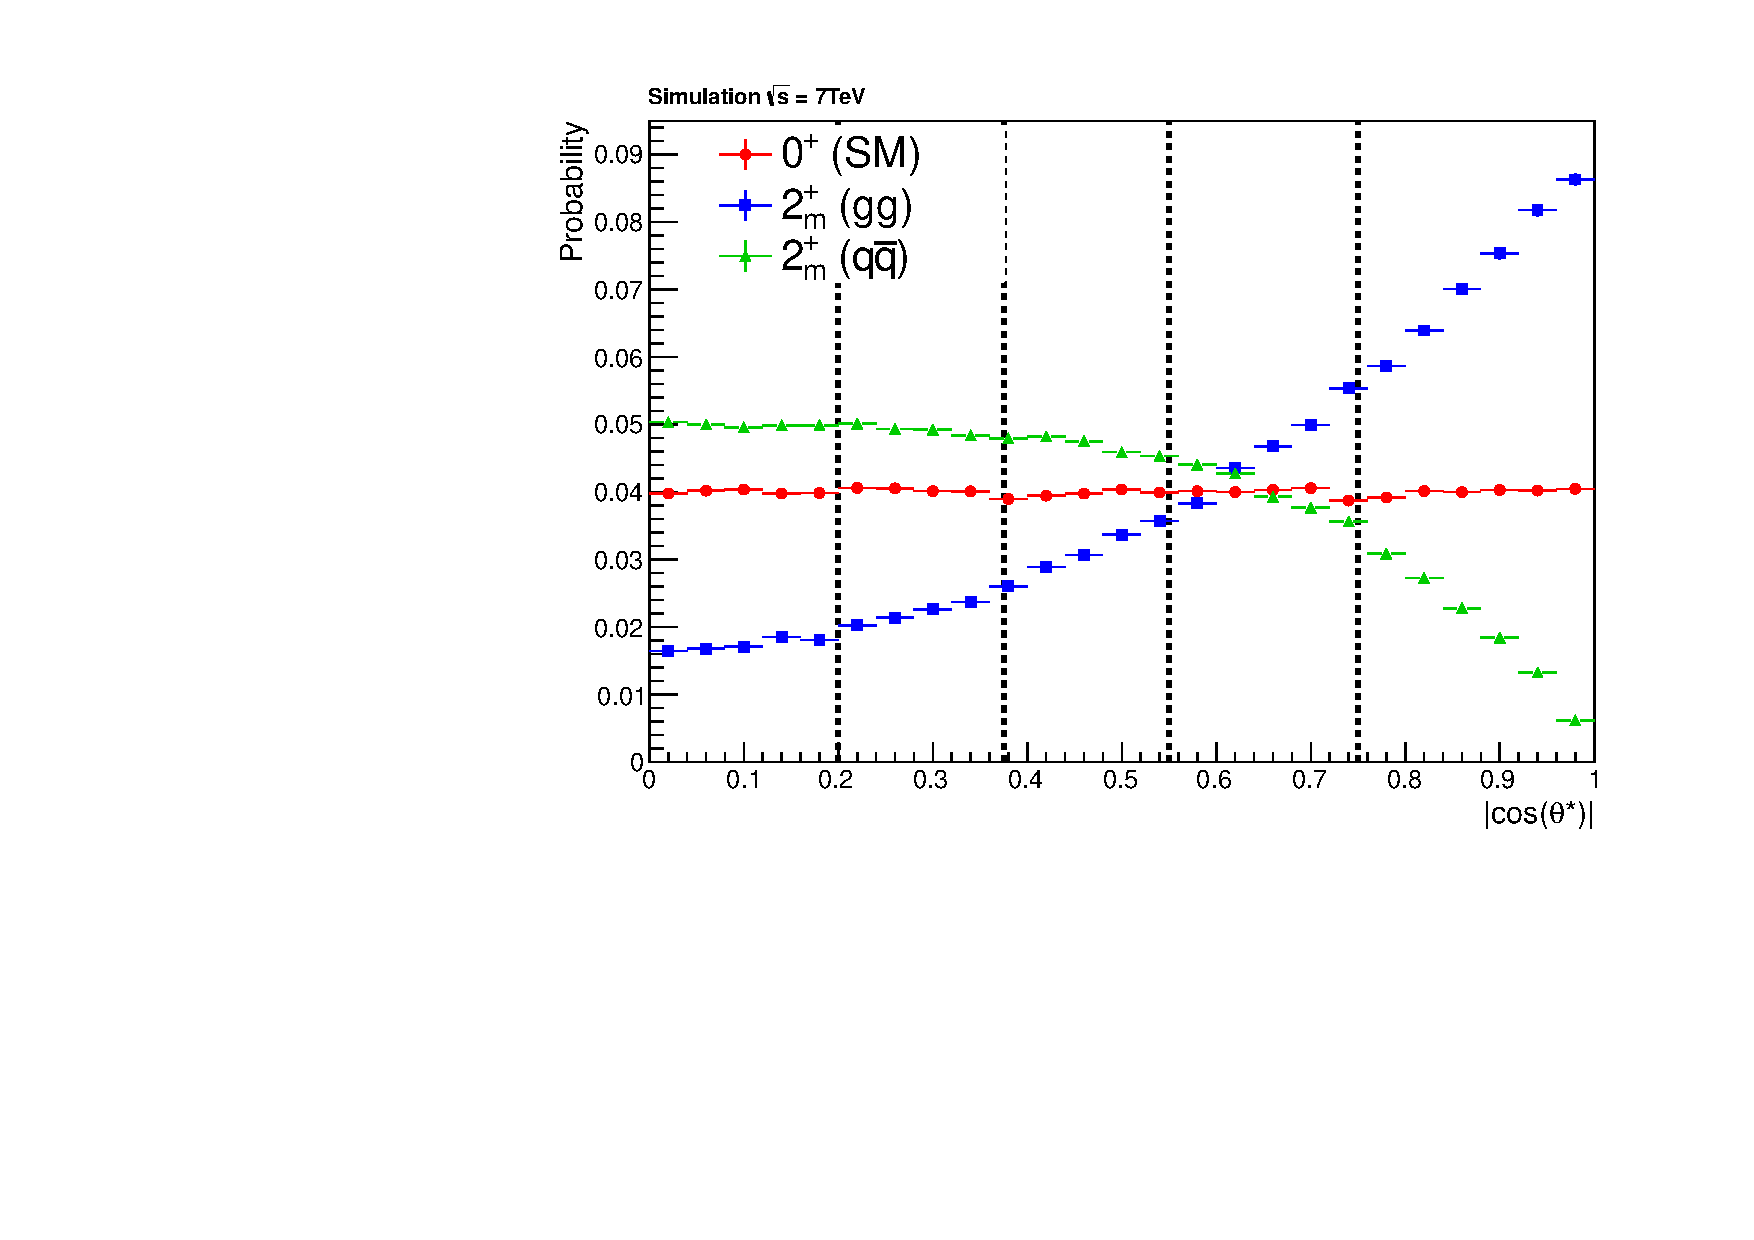
\includegraphics[width=0.49\linewidth]{analysis/plots/spin/before_7TeV.pdf}
	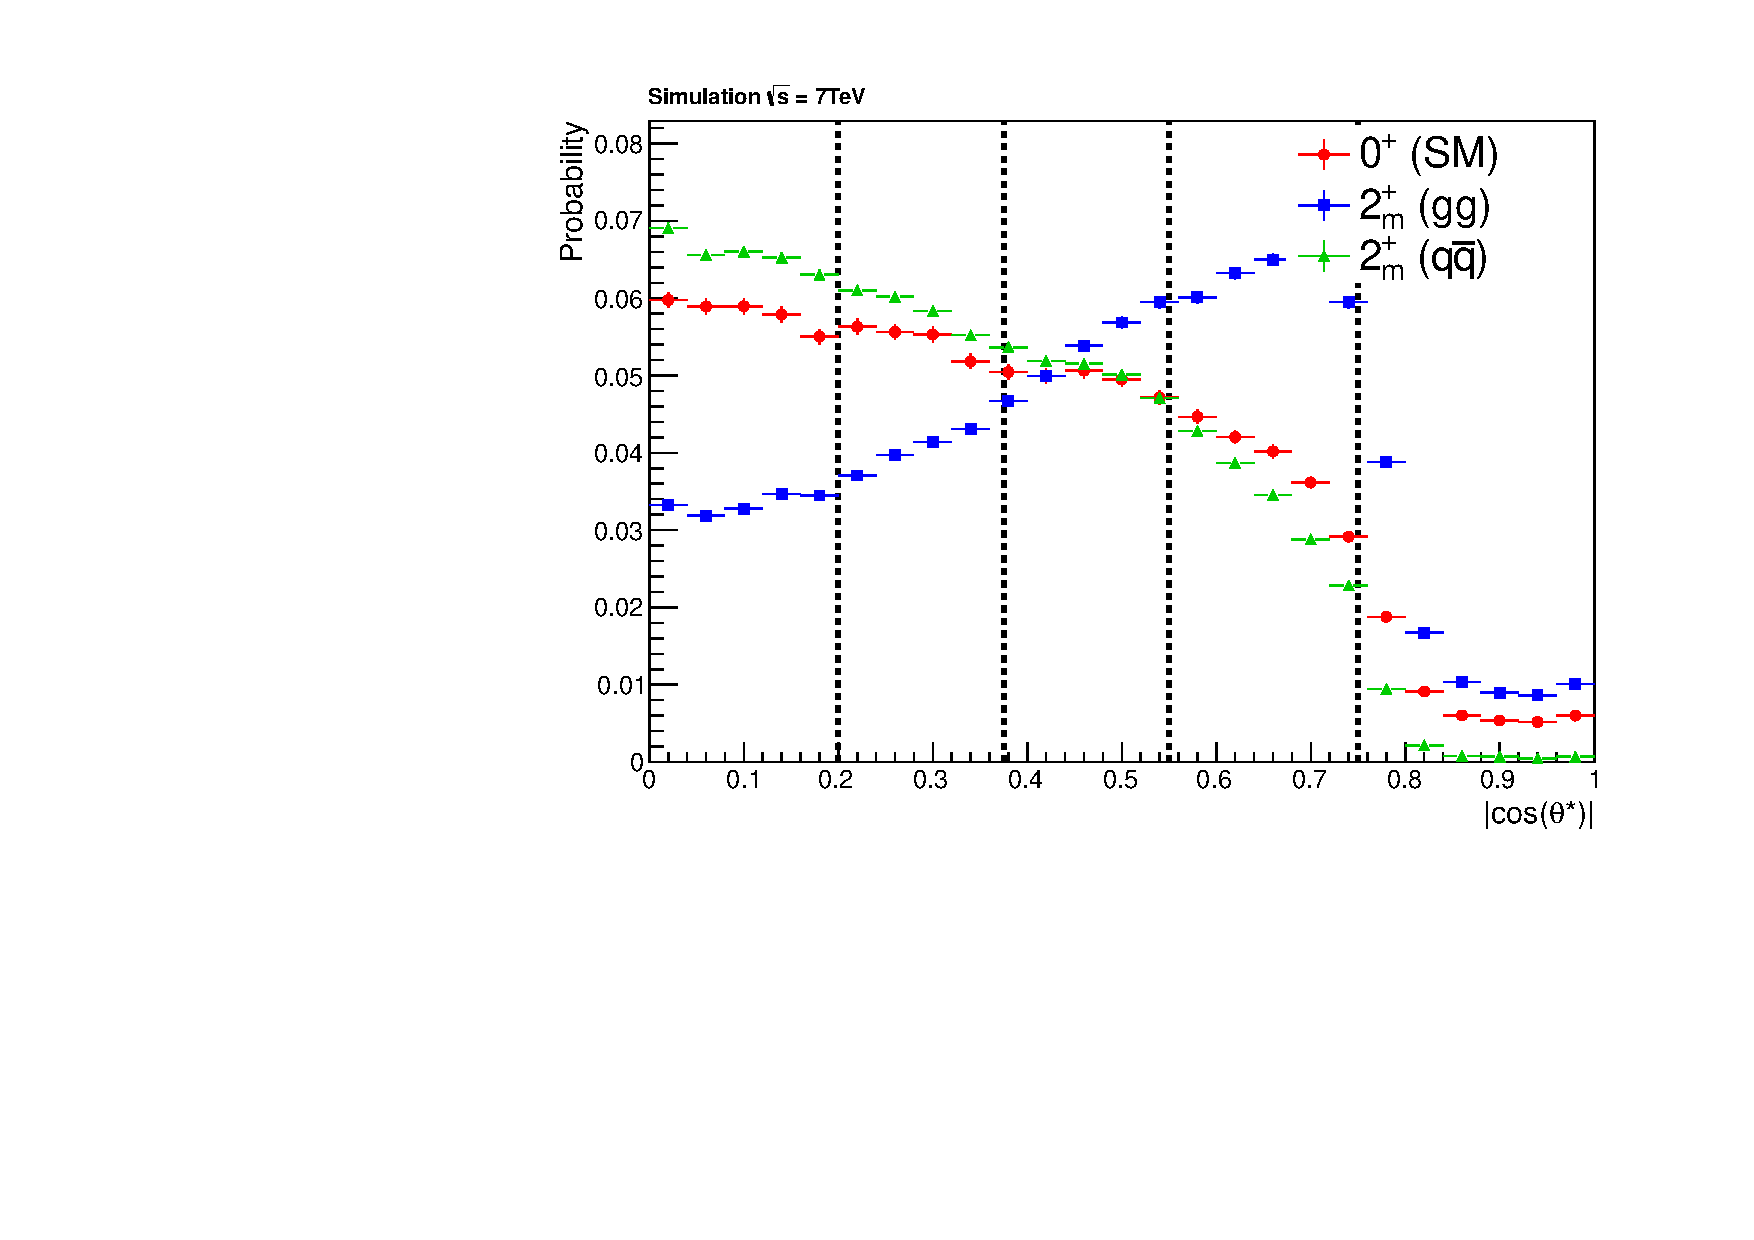
\includegraphics[width=0.49\linewidth]{analysis/plots/spin/after_7TeV.pdf} \\
	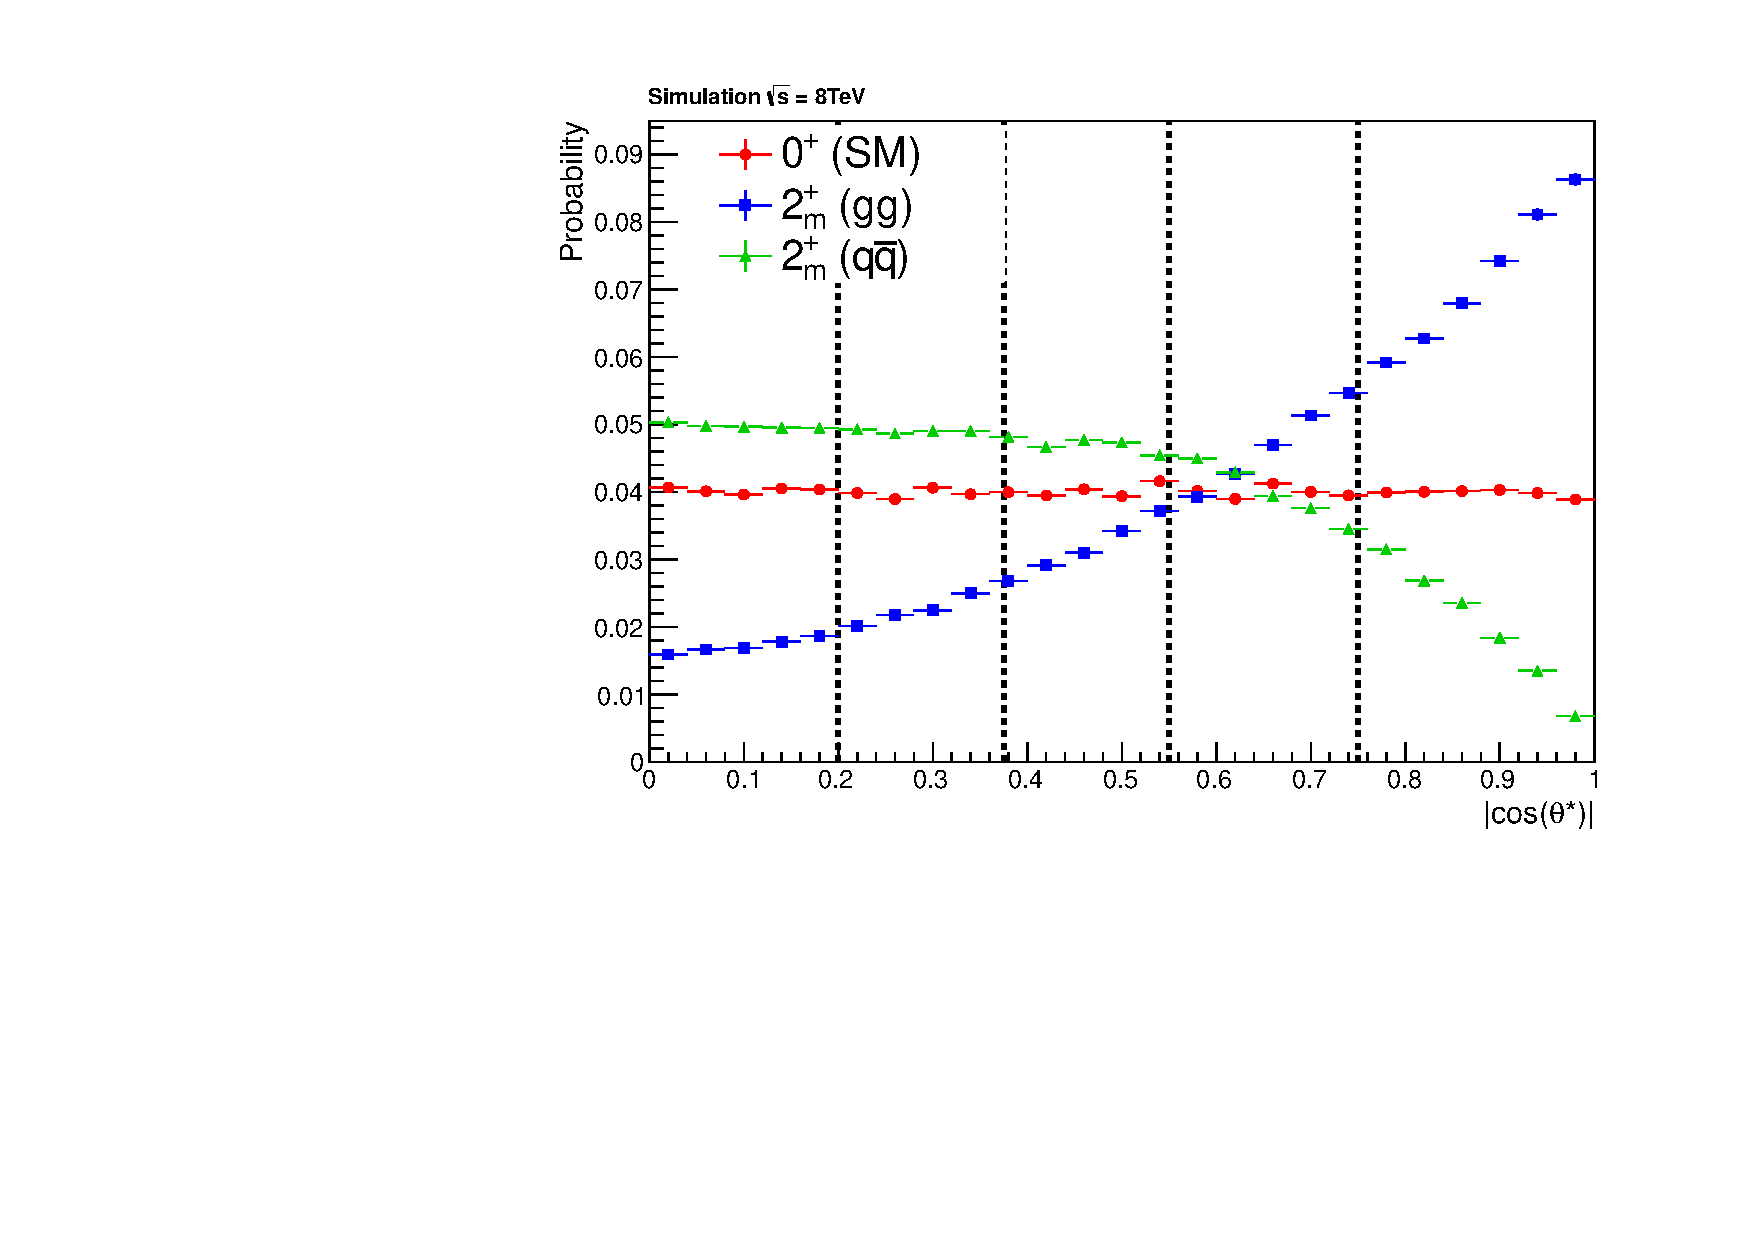
\includegraphics[width=0.49\linewidth]{analysis/plots/spin/before_8TeV.pdf}
	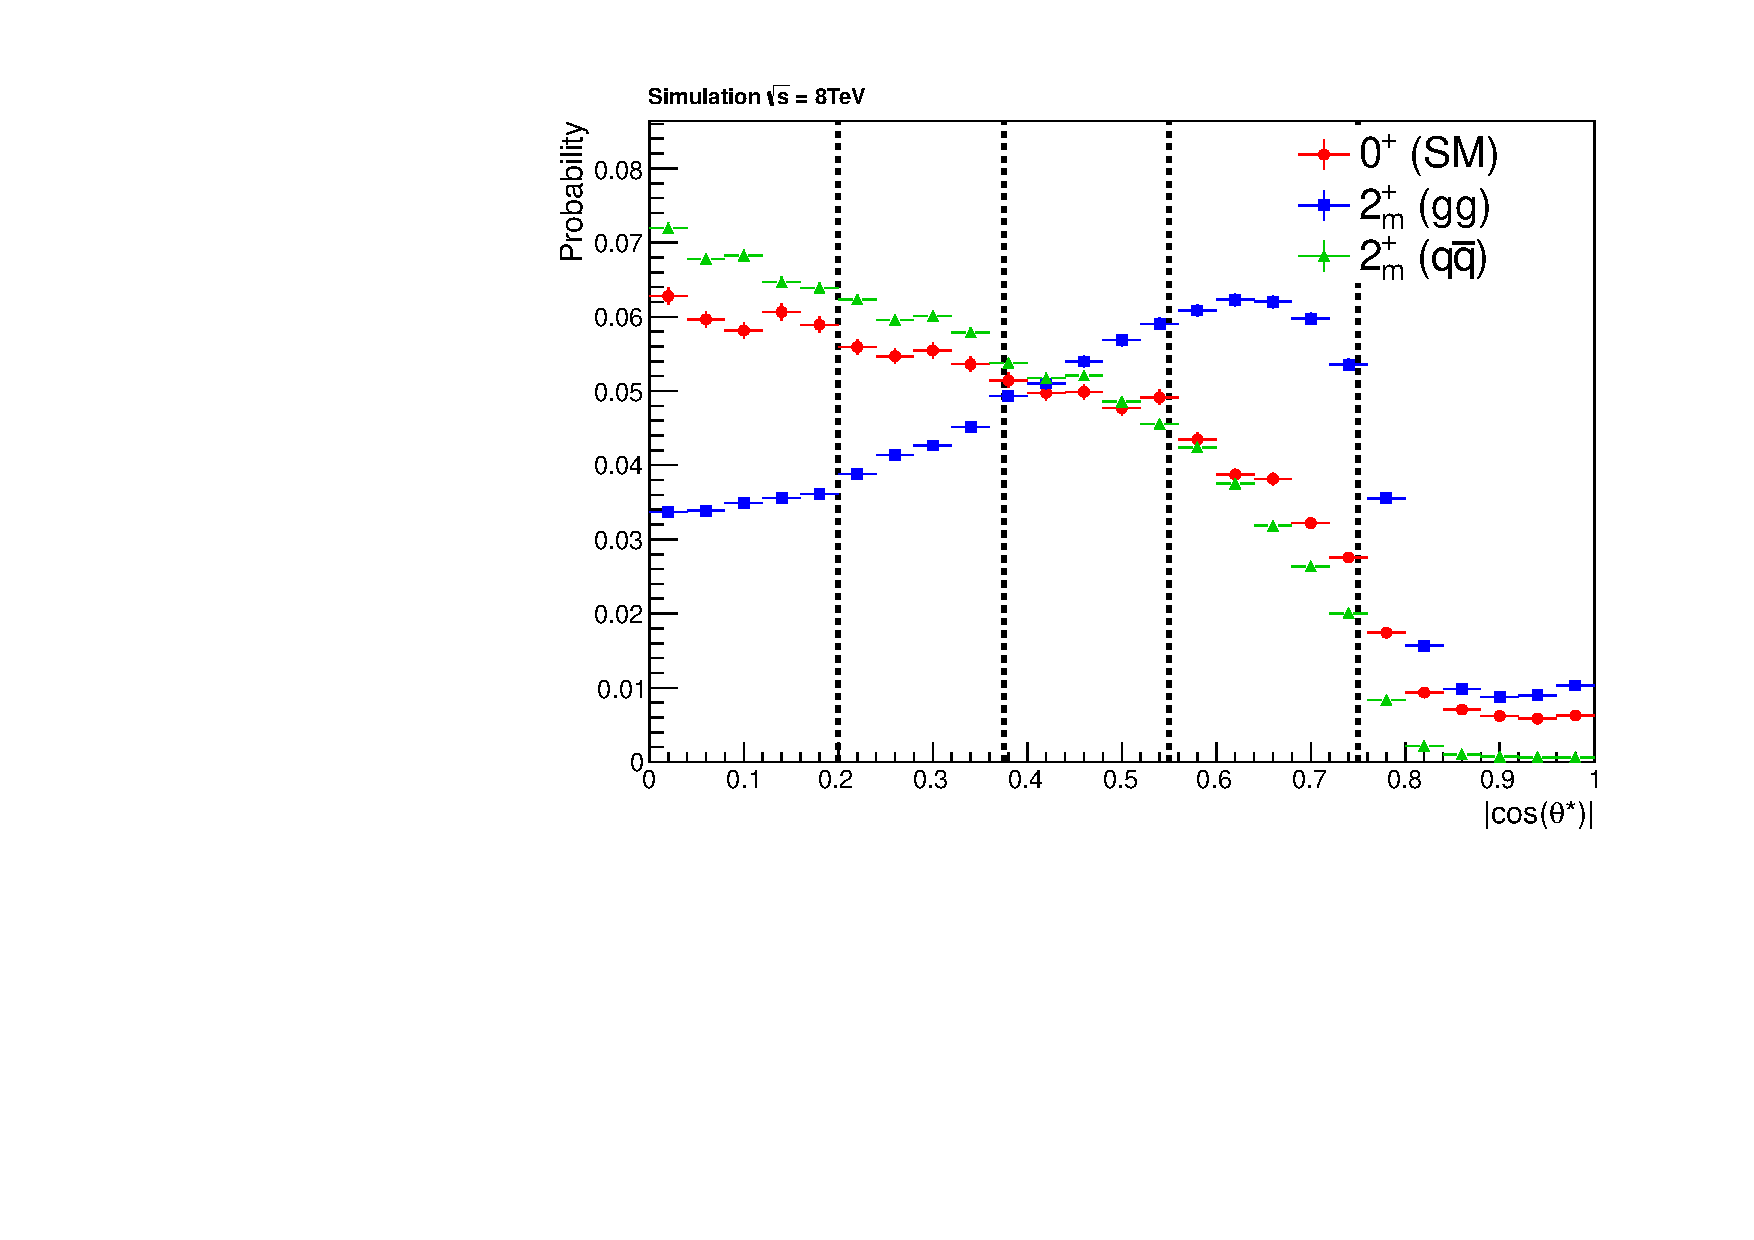
\includegraphics[width=0.49\linewidth]{analysis/plots/spin/after_8TeV.pdf} \\
	\caption[The distribution of \abscostheta before and after selection cuts for different spin signals]{The distribution of \abscostheta before any selection cuts (left) and after the selection cuts (right) for the 7~\TeV dataset (top row) and the 8~\TeV dataset (bottom row). The three histograms represent the spin $0^+$ distribution with all SM production modes (red circular points), the spin $2^+_m$ distribution with the gluon-fusion production mode (blue square points) and the spin $2^+_m$ distribution with the quark-antiquark annihilation production mode (green triangular points). The \abscostheta category boundaries are shown as the black dashed lines.}
	\label{fig:acc_cuts}
	\end{center}
\end{figure}	

A robust analysis is possible because although the acceptance $\times$ efficiency varies considerably as a function of \abscostheta, the shape of this variation is largely independent of the spin-parity model. This is also true in restricted ranges of $\eta$ and $R_{9}$ which allows us to extract the signal yield in bins of \abscostheta in a comparatively model independent way. 
Figure~\ref{fig:eff_acc} shows the efficiency $\times$ acceptance ratio between the \twomp (with gluon-fusion production only) and \zerop (all SM production modes) as a function of \abscostheta in the $|\eta|$ and $R_{9}$ categories defined in Table~\ref{table:cats1}. It is clear that the acceptance $\times$ efficiency between the spin-0 and spin-2 models is independent of \abscostheta apart from at high values of \abscostheta where the vector boson-fusion production in the SM plays a role. This motivates the choice of \abscostheta category boundaries described below where all the categories have similar efficiency $\times$ acceptance apart from the bin highest in \abscostheta.

\begin{figure}
	\begin{center}
	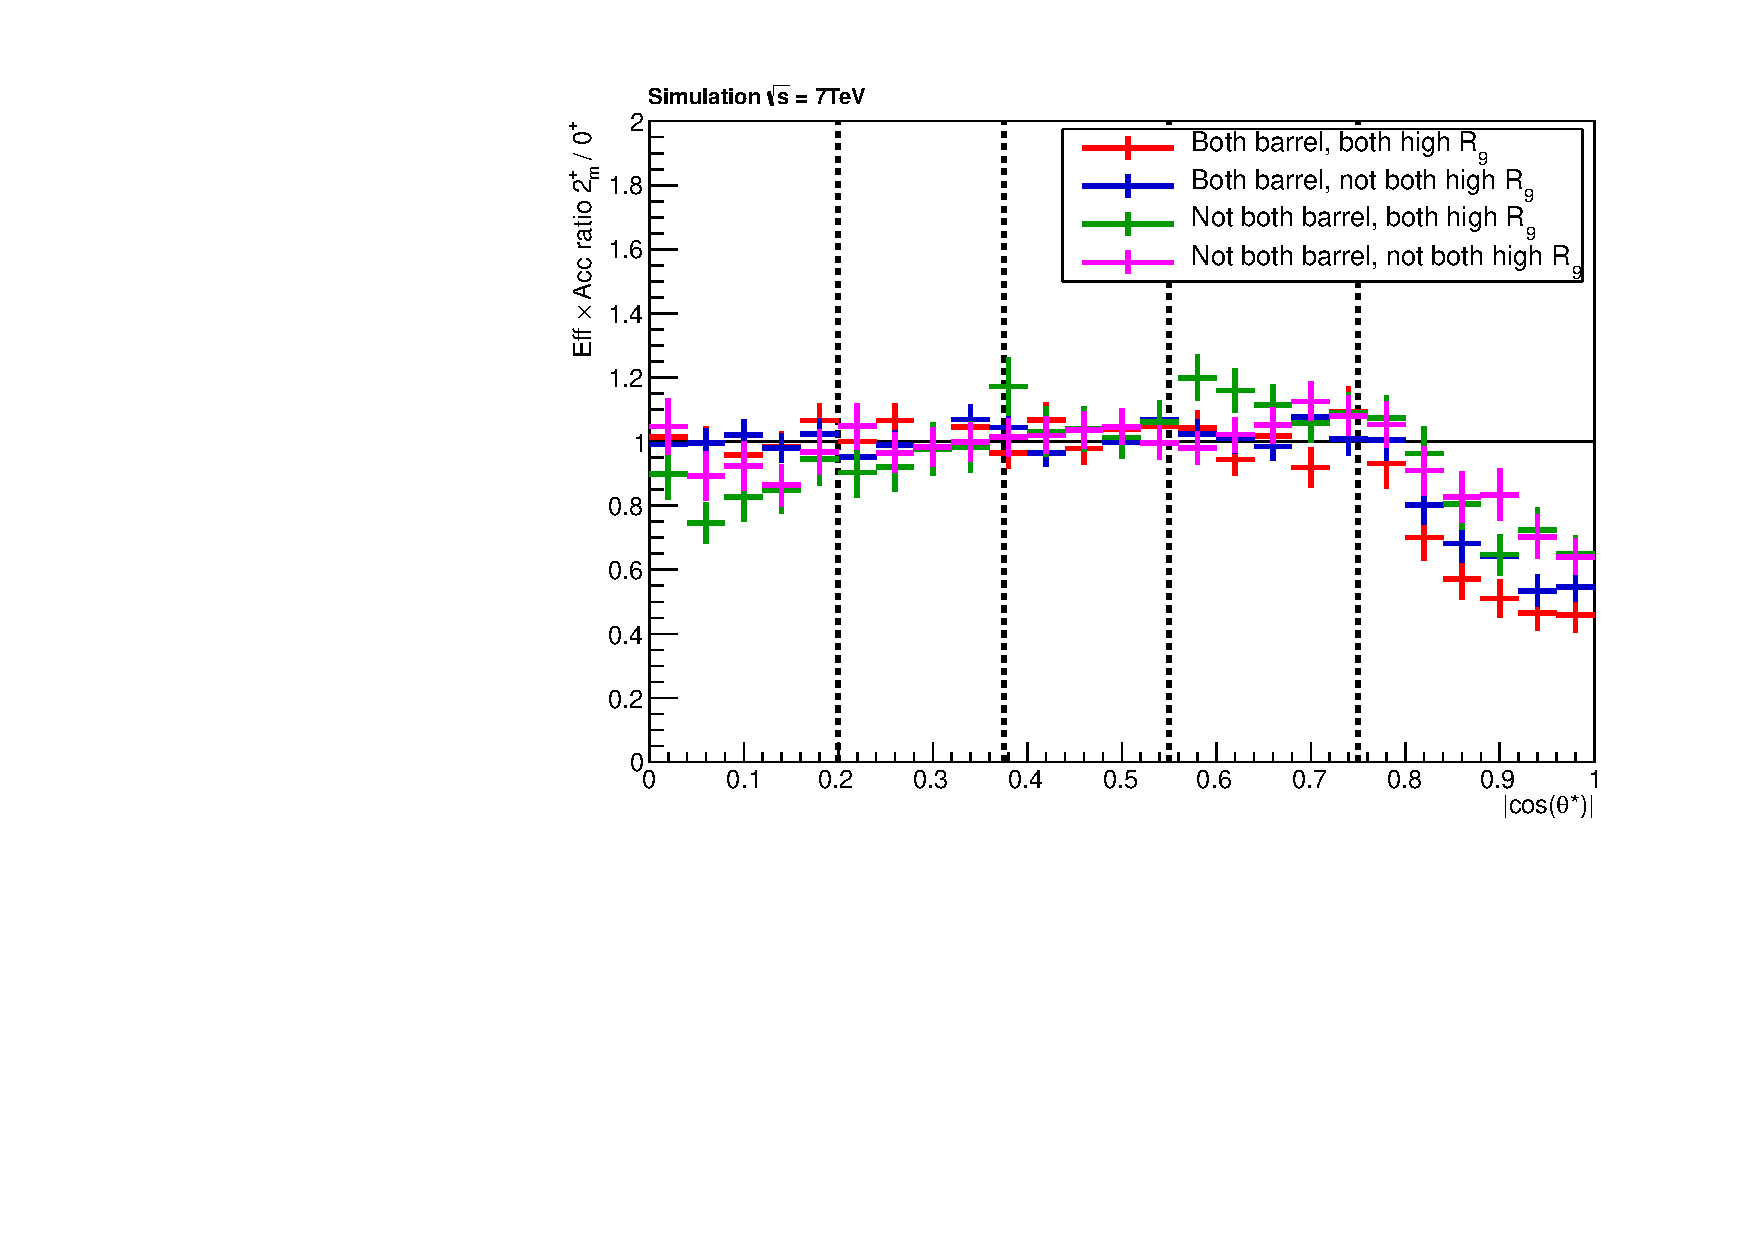
\includegraphics[width=0.49\linewidth]{analysis/plots/spin/effacccats_7TeV.pdf}
	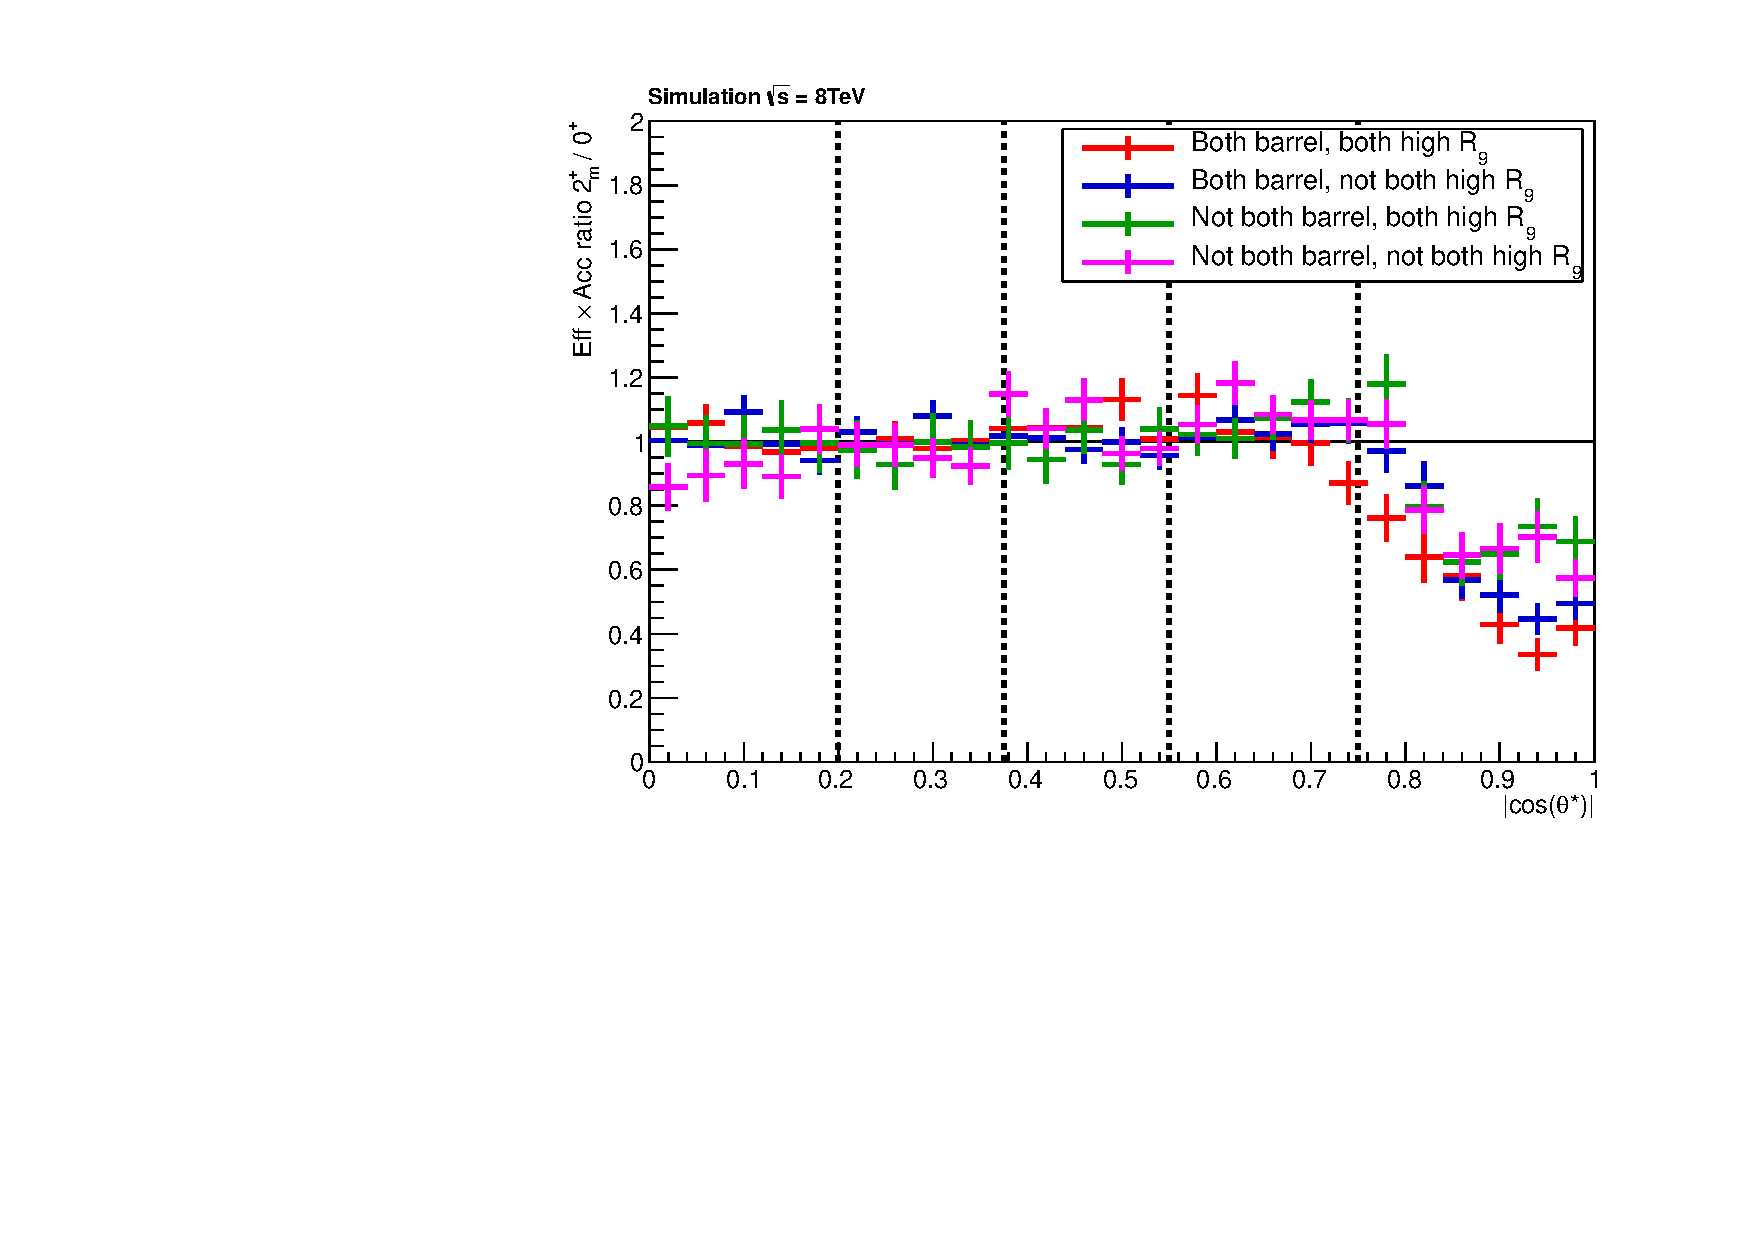
\includegraphics[width=0.49\linewidth]{analysis/plots/spin/effacccats_8TeV.pdf}
  \caption[Acceptance $\times$ efficiency ratio between the \twomp (gluon fusion production) and \zerop (all SM production modes) of the spin analysis event selection]{Acceptance $\times$ efficiency ratio between the \twomp (gluon-fusion production) and \zerop (all SM production modes) of the event selection as a function of \abscostheta split into the $|\eta|$ and $R_{9}$ categories defined in Table~\ref{table:cats1}. The \abscostheta category boundaries are shown as the black dashed lines. The left hand plot is for the 7~\TeV and the right hand plot for the 8~\TeV.}
	\label{fig:eff_acc}
	\end{center}
\end{figure}	

To benefit from the improved energy resolution of non-showering photons in 
the barrel, each event is categorised in $\eta$ and $R_{9}$ according to Table~\ref{table:cats1}.

\begin{table}
  \begin{center}
    \caption[Definition of the photon resolution categories in the spin analysis]{Definition of the photon resolution categories in the spin analysis. Here $|\eta|_{\mbox{\tiny{max}}}$ and $R_{9\mbox{\tiny{min}}}$ refer to the maximum $\eta$ and minimum $R_{9}$ of the two photons.}
    \begin{tabular}{ l | l l l }
      Category 0 & $|\eta|_{\mbox{\tiny{max}}}<1.444$ & and & $R_{9\mbox{\tiny{min}}}\geq0.94$ \tabularnewline 
      Category 1 & $|\eta|_{\mbox{\tiny{max}}}<1.444$ & and & $R_{9\mbox{\tiny{min}}}<0.94$ \tabularnewline 
      Category 2 & $|\eta|_{\mbox{\tiny{max}}}>1.556$ & and & $R_{9\mbox{\tiny{min}}}\geq0.94$ \tabularnewline 
      Category 3 & $|\eta|_{\mbox{\tiny{max}}}>1.556$ & and & $R_{9\mbox{\tiny{min}}}<0.94$ \tabularnewline
    \end{tabular}
    \label{table:cats1}
  \end{center}
\end{table}

%\begin{tabular}{l l l l l}
%  \textbullet & Category 0: & $|\eta|_{\mbox{\tiny{max}}}<1.444$ & and & $R_{9\mbox{\tiny{min}}}>0.94$ \\ 
%  \textbullet & Category 1: & $|\eta|_{\mbox{\tiny{max}}}<1.444$ & and & $R_{9\mbox{\tiny{min}}}\leq0.94$ \\ 
%  \textbullet & Category 2: & $|\eta|_{\mbox{\tiny{max}}}>1.444$ & and & $R_{9\mbox{\tiny{min}}}>0.94$ \\ 
%  \textbullet & Category 3: & $|\eta|_{\mbox{\tiny{max}}}>1.444$ & and & $R_{9\mbox{\tiny{min}}}\leq0.94$ \\
%\end{tabular}

Within each category events are binned in \abscostheta, to discriminate between the different spin hypotheses, according to Table.~\ref{table:cats2}.

\begin{table}
  \begin{center}
    \caption{Definition of diphoton \abscostheta categories in the spin analysis.}
    \begin{tabular}{ l | r l }
      Spin Category 0 &             & \abscostheta $<0.2$ \tabularnewline 
      Spin Category 1 & $0.2\leq$   & \abscostheta$<0.375$ \tabularnewline 
      Spin Category 2 & $0.375\leq$ & \abscostheta$<0.55$ \tabularnewline 
      Spin Category 3 & $0.55\leq$  & \abscostheta$<0.75$ \tabularnewline 
      Spin Category 4 & $0.75\leq$  & \abscostheta$<1.0$ \tabularnewline 
    \end{tabular}
    \label{table:cats2}
  \end{center}
\end{table}

The \abscostheta boundaries are optimised to make particular use of the most disciminating 
bin (high \abscostheta) and to maintain uniform acceptance $\times$ efficiency in the 
other bins. In total the analysis is split into 20 event classes (4 $\eta$/\rnine\xspace 
categories $\times$ 5 \abscostheta categories) in each year which gives a total of 40 event classes.

\subsection{Event categorisation summary}

All the categories and the tagging order are summarised in Table~\ref{tab:cat_summary}.

\begin{table}[h!]
\caption{The event classes at 7 and 8~\TeV and some of their main selection requirements. Events are tested against the selection requirements
of the classes in the order they are listed here.}
\begin{center}
\begin{tabular}{l c c p{10cm}}
\multirow{2}{*}{Label} & \multicolumn{2}{l}{No. of classes} & \multirow{2}{*}{Main requirements} \\
 & 7~\TeV & 8~\TeV & \\
\hline
\multirow{3}{*}{\ttH lepton tag} & \multirow{3}{*}{$\star$} & \multirow{3}{*}{1} & $\ptgom>1/2$ \\ %% $\text{diphoton BDT}>-0.6$
                                                                               & & & 1 b-tagged jet + 1 electron or muon \\
                                                                               & & & diphoton BDT $>0.6(-0.6)$ at 7(8)~\TeV \\
\hline
\multirow{4}{*}{\VH tight $\ell$ tag} & \multirow{4}{*}{1} & \multirow{4}{*}{1} & $\ptgom>3/8$ \\ %% $\text{diphoton BDT}>-0.6$
                                                                  & & & $e$ or $\mu$, $\pT>20$~\GeV, and $\MET>45$~\GeV OR\\
                                                                  & & & $2e$ or $2\mu$, $\pT>10$~\GeV; $70<m_{ll}<110$~\GeV \\
                                                                  & & & diphoton BDT $>0.1(-0.6)$ at 7(8)~\TeV \\
\hline
\multirow{3}{*}{\VH loose $\ell$ tag} & \multirow{3}{*}{1} & \multirow{3}{*}{1} & $\ptgom>3/8$ \\ %%  $\text{diphoton BDT}>-0.6$
                                                                   & & & $e$ or $\mu$, $\pT>20$~\GeV \\
                                                                   & & & diphoton BDT $>0.1(-0.6)$ at 7(8)~\TeV \\

\hline
\multirow{3}{*}{\VBF dijet tag} & \multirow{3}{*}{2} & \multirow{3}{*}{3} & $\ptgom>1/2$\\
                                                                             & & & 2 jets; dijet and combined diphoton-dijet BDTs used\\
\hline
\multirow{3}{*}{\VH \MET\ tag} & \multirow{3}{*}{1} & \multirow{3}{*}{1} & $\ptgom>3/8$ \\ %% , $\text{diphoton BDT}>0.0$ 
                                                                    & & & $\MET>70$~\GeV \\
                                                                    & & & diphoton BDT $>0.8(0.0)$ at 7(8)~\TeV \\ 

\hline
\multirow{3}{*}{\ttH multijet tag} & \multirow{3}{*}{$\star$} & \multirow{3}{*}{1} & $\ptgom>1/2$ \\ %% , $\text{diphoton BDT}>-0.3$
                                                                       & & & 1 b-tagged jet + 4 more jets \\
                                                                       & & & diphoton BDT $>0.6(-0.2)$ at 7(8)~\TeV \\ 
\hline
\multirow{3}{*}{\VH dijet tag} & \multirow{3}{*}{1} & \multirow{3}{*}{1} & $\ptgom>3/8$\\ %% , $\text{diphoton BDT}>0.2$ 
                                                                                         & & & jet pair, $\pT>40$~\GeV and $60<\mjj<120$~\GeV \\
                                                                                         & & & diphoton BDT $>0.6(0.2)$ at 7(8)~\TeV \\ 

\hline
\multirow{3}{*}{Untagged} & \multirow{3}{*}{4/8/20$^{\dagger}$} & \multirow{3}{*}{5/10/20$^{\dagger}$} & The remaining events,\\
                                                                          & &  & classified using diphoton BDT \\
\hline
\multicolumn{4}{ p{16cm} }{$\star$ For the 7~\TeV dataset, events in the \ttH lepton tag and multijet tag classes are combined,
after selection, to form a single event class.} \\
\multicolumn{4}{ p{16cm} }{$\dagger$ For the \MFM there are 4 (5) categories at 7 (8)~\TeV, for the \SMVA there are 8 (10) and for the spin analysis there are 20 (20) with no exclusive categories.} \\
\end{tabular}
\end{center} 
\label{tab:cat_summary}
\end{table}

%\begin{table}[h!]
%  \begin{center}
%    \begin{tabular}{l | l l l l l l}
%      \multirow{3}{*}{Category type} & \multicolumn{6}{c}{Number of categories} \\
%      & \multicolumn{2}{c}{\CiC} & \multicolumn{2}{c}{\MFM} & \multicolumn{2}{c}{\SMVA} \\
%      & 7~\TeV & 8~\TeV & 7~\TeV & 8~\TeV & 7~\TeV & 8~\TeV \\
%      \hline
%      Inclusive & 8 & 8 & 4 & 5 & 8 & 10 \\
%      \VBF tagged & 2 & 2 & 2 & 3 & 2 & 3 \\
%      \VH tagged & 4 & 4 & 4 & 4 & 4 & 4 \\
%      \ttH tagged & 1 & 2 & 1 & 2 & 1 & 2 \\
%    \end{tabular}
%    \caption{A summary of the number of categories for each of the analyses.}
%    \label{tab:cat_summary}
%  \end{center}
%\end{table}
